% Numerics tables and figure for the weil-edge paper. % Numerics tables and figure for the weil-edge paper. % Numerics tables and figure for the weil-edge paper. % Numerics tables and figure for the weil-edge paper. \input{numerics/tables} from papers/weil-edge/.
% Needs: booktabs, array, amsmath, graphicx. The tabulars tab_kink_*.tex, tab_k5.tex, tab_tail_*.tex are generated by
% make_tables.py from data; tab_detect.tex, tab_H.tex and tab_cX.tex are copied by hand from the sources in numerics.md.
% Statement labels follow the synthesis note: K1 (edge law to second order, D = lambda + log 2pi + gamma),
% K3 (first-order kink profile), K6 (jump-ratio offset with prime-power boosts), T2 (first-order tail law),
% T4 / Pred. F (lambda-shifted second-order tail law). Registered IDs of the pre-registration in brackets.

\begin{table}[p]\centering\footnotesize\setlength\tabcolsep{3pt}
\input{numerics/tab_detect}
\caption{Which numerical checks can detect a wrong constant. The exact identities (N1--N5) hold for any value $\kappa$ of the layer constant in Lemmas~8.2--8.3, so they cannot confirm the constant $2$ in (H); only absolute determinations of $A$ compared with $\lambda'$ can. ``Yes'' gives the size of error the check would see. Nothing here is certified, and nothing here bears on the Riemann hypothesis.}\label{tab:detect}
\end{table}

\begin{table}[p]\centering\footnotesize\setlength\tabcolsep{3pt}
\input{numerics/tab_H}
\caption{Absolute checks of the constant in (H): $-\lambda'/(2A^2)$, predicted to be $1$. P0: the piecewise-constant Galerkin code of the final internal referee, independent of the project's hp-FEM; edge mesh down to $r=10^{-150}$, $A$ fitted on $\ell\in[30,345]$ and extrapolated in the grading ratio. ``Refined'' adds the measured shift from $h_0=L/500$ to $L/2000$ (contrast row: $h_0=L/1000$). The $L=0.6$ odd entry is the weakest ($\lambda'$ from one mesh while $\lambda_o$ moves by $2\%$ under refinement). Fitted amplitudes with active primes carry an extra resolution bias of $0.15$--$0.3\%$ unless the mesh is graded at $\pm(L-\log n)$ (contrast row). The pure-log case is treated in the companion paper; it is listed only because it is one of the absolute checks. hp-FEM N9 has one exception, the true even ground state at $L=0.7$ ($\lambda'=-3.5\cdot10^{-11}$, at the double-precision floor, ratio $0.9915$).}\label{tab:H}
\end{table}

\begin{table}[p]\centering\footnotesize\setlength\tabcolsep{2.5pt}
\input{numerics/tab_kink_gen1}
\caption{Generation-1 kink constants (K3 with $k=1$; registered K1). Fits $\mathsf J\ell^{3/2}/(c_nA)=\kappa_0+\kappa_1/\ell+\kappa_2/\ell^2$ and $\psi(q-r)+\psi(q+r)=2\psi(q)+c_nA\ell^{-3/2}(\sigma_0+\dots)$ on $\ell\in[20,\ell_{\max}-6]$, finest grading; side $=(\kappa_0+\sigma_0)/(\sigma_0-\kappa_0)$. Predictions in the headers. ``rows'': chain points $y_n$, $n<X$ (at $L=0.6$ with mirrors). Brackets give the range over rows; $\pm$ is a systematic band, not a standard deviation: the spread over grading ratios plus the change when the fit window starts at $\ell=15$ or $25$ instead of $20$ (\texttt{kink\_errors.out}). Original registered verdict on every row: PASS (50/50 graded rows; tolerances $0.005$, $0.003$, $0.015$). $^\dagger$Post-registration diagnostic, all coupled generation-2 points graded; not a registered verdict. $^\ddagger$The new pre-registered rerun (Table~\ref{tab:k5}), primary meshes; PASS 10/10 under the same tolerances (also with $\rho=1.15$ added).}\label{tab:kink1}
\end{table}

\begin{table}[p]\centering\footnotesize\setlength\tabcolsep{3pt}
\input{numerics/tab_kink_gen2}
\caption{Generation-2 kink constants (K3 with $k=2$; registered K2): predicted jump coefficient $1$, cusp $\frac15$ and side ratio $-\frac32$, i.e.\ the split $\frac35:-\frac25$, with chain weight $W$ ($c_2c_3=0.3109$, $c_3c_4=0.2198$, $2c_2c_3=0.6218$). Same fits and error bands as Table~\ref{tab:kink1}. Original registered verdict: PASS 20/20 (tolerances $0.01$, $0.004$, $0.015$). $^\dagger$Post-registration diagnostic. $^\ddagger$New pre-registered rerun, primary meshes; PASS 2/2. In the rerun the generation-3 point $L-\log\frac65$, coupled to $L-\log6$, is also graded.}\label{tab:kink2}
\end{table}

\begin{table}[p]\centering\footnotesize\setlength\tabcolsep{3pt}
\input{numerics/tab_k5}
\caption{Jump-ratio offset (K6; registered K5). Prediction: $1/\rho_n-\ell\to-D-\beta_n$, with $\rho_n=\mathsf J/(c_n\psi(L-r))$, $D=\lambda+\log2\pi+\gamma$ and boosts $\beta_n=W_2^+(y_n)/c_n$; at $L=0.6$ the prime power $4$ is not active, so every boost vanishes there. Registered pass rule (tolerance $0.005$): the grading-extrapolated $b_0+D+\beta_n$ \emph{and} the calibration-free $|b_0+D_{\rm fit}+\beta_n|$ at every grading. $\pm$: fit-window band plus, where three gradings exist, the spread of the two two-mesh extrapolations; with two gradings the extrapolation has no internal check. ``reg.'': the registered $L=1.0$ mesh, generation-2 points graded only to $10^{-16}$ ($\ell=36.8$, inside the fit window $[20,63]$). ``sens.'': the registered sensitivity mesh, one grading only (raw value, no extrapolation). These two meshes give the registered FAIL on 17 of the 20 graded $L=1.0$ rows; it stays in the record. $^\dagger$Post-registration diagnostic; its second mesh had a shorter fit window, so the calibrated column shows the $\rho=1.5$ value and no verdict is given. $^\ddagger$New pre-registered rerun (\texttt{PREREG\_K5\_L1.md}): every chain point coupled to a measured point graded through the whole fit window; primary verdict on $\rho\in\{1.5,1.25\}$, supplementary with $\rho=1.15$ added.}\label{tab:k5}
\end{table}

\begin{table}[p]\centering\footnotesize\setlength\tabcolsep{3pt}
\input{numerics/tab_k0}
\caption{Edge law to second order (K1; registered K0$'$): $\psi(L-r)=A(\ell-D)^{-1/2}+O(\ell^{-5/2})$, $D=\lambda+\log2\pi+\gamma$. $D_{\rm fit}=-a_1/a_0$ from $\psi(L-r)^{-2}=a_0\ell+a_1+a_2/\ell+a_3/\ell^2$ on $\ell\in[20,\ell_{\max}-6]$, extrapolated in the grading ratio; tolerance $0.005$. The deviation is positive in every row, so a small systematic offset of the fit model (up to about $0.005$) cannot be excluded; it is of the size of the fit-window band. In the new rerun the odd $s=5$ state fails this registered test by $1\cdot10^{-4}$ (primary) and $5\cdot10^{-6}$ (supplementary), well inside its band $\pm0.003$; it passed ($+0.0047$) on the registered mesh. Labels as in Table~\ref{tab:k5}.}\label{tab:k0}
\end{table}

\begin{table}[p]\centering\scriptsize\setlength\tabcolsep{2.5pt}
\input{numerics/tab_tail_T1}
\caption{Tail law, second order (T4 / Pred.~F; registered T1, T1-full, T1-$\lambda$) on actual zeta zeros ($\gamma\le10\,303$, Arb). Columns: $Z/P_1$ on four of the seven blocks, where $Z$ is the zero-side block sum and $P_1=(|\lambda'|/\pi)\int(a+\varepsilon c_X)/(t^2(a-\lambda))$; the range of $\tau/\tau_{\rm pred}-1$ for $T\ge400$; and $Z/P$ without the $\lambda$-shift, first to last block. ``mesh'': largest fine-versus-base block difference (the numerical error of $Z$). The deviations from $1$ are not numerical error: they are the unmodelled $O(a^{-2})$ remainder, always negative, of the order of $\sum_{n<X}c_n^2/a^2$. The registered tolerance was generous ($0.13$--$0.21$ on $[400,800]$); every graded state passed inside it by at least a factor $2$. States: ground states of their sector at pole strength $s$ (E0: $s=0$, Em1: $s=-1$, O5: $s=5$, O20: $s=20$); large $|\lambda|$, so these test the theorems where $\lambda/\log T$ is large, not the true $s=1$ form at small $\lambda$.}\label{tab:T1}
\end{table}

\begin{table}[p]\centering\footnotesize\setlength\tabcolsep{3pt}
\input{numerics/tab_tail_T2}
\caption{Sector split (registered T2): fit of $S_k=\ln(Z_e/E_e)_k-\ln(Z_o/E_o)_k=\alpha\langle1/a\rangle_k+\beta\langle a^{-2}\rangle_k$ over six blocks; prediction $\alpha=2c_X$. Registered pass rule $|\alpha-2c_X|\le\max(0.10,3\sigma_\alpha)$. At $X=8$ two pairs are $2.6\sigma$ and $3.0\sigma$ high; the second passes the $3\sigma$ rule by less than $0.003$. The $X=10$ control lies between $0$ and $2c_8$ and does not discriminate. At $T\le10^4$ the $1/a$ split cannot be separated cleanly from the $a^{-2}$ kink terms.}\label{tab:T2}
\end{table}

\begin{table}[p]\centering\footnotesize\setlength\tabcolsep{3pt}
\input{numerics/tab_cX}
\caption{The $\pm c_X$ term at prime-power $X=e^{2L}$, on actual zeros. $X=2,3$: no $nm=X$ competition, the cleanest test (P0 eigenfunctions, $-\lambda'/2A^2=0.995$--$0.999$). $X=4$: even sector only; the odd state there has $|A|\sim0.02$ and $\lambda_o$ is not mesh-converged, and the derivative-free split matches $2c_4\langle1/a\rangle$ only within $10$--$30\%$. $X=8$: pre-registered (Table~\ref{tab:T2}). The post-hoc row compares $Z/P_0$ across $X$ for states of the same kind; the states differ in $\lambda$. The $c_X$ term is supported at $X=2,3,4,8$; at $X=8$ it is not cleanly separated from the $\ell^{-2}$ kink terms.}\label{tab:cX}
\end{table}

\begin{figure}[p]\centering
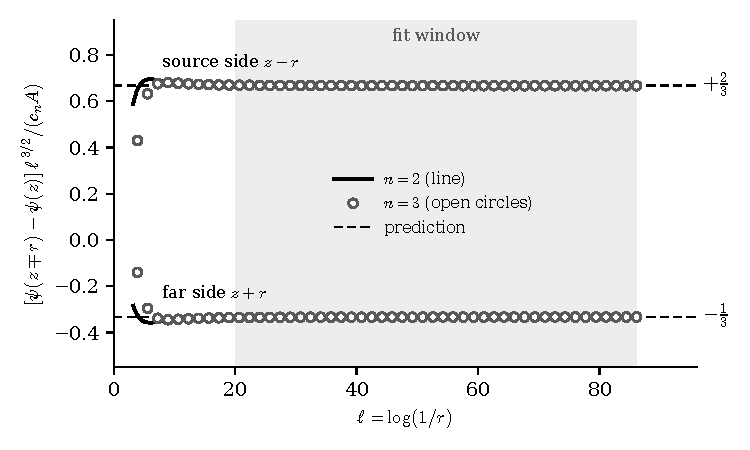
\includegraphics[width=0.8\textwidth]{numerics/fig_kink_split.pdf}
\caption{Generation-1 kink profile at $L=0.6$ (even ground state, $s=0$, $\lambda=-2.417$, $A=1.567$; P1, grading $\rho=1.15$ down to $r=10^{-40}$). Plotted: the one-sided excursions $[\psi(q\mp r)-\psi(q)]\ell^{3/2}/(c_nA)$ at $q=y_n=L-\log n$, with $\psi(q)$ from the cusp fit (the node value at $q$ itself is truncated). Dashed: the predicted split $+\frac23$ (source side) and $-\frac13$ (far side) of K3. Line: $n=2$; circles: $n=3$ (every 12th node). The two coincide because $D\approx-0.002$ and $\beta_2=\beta_3=0$ here, so the $O(1/\ell)$ correction nearly vanishes. Fitted limits: $0.66679$ and $-0.33335$ for both points. Data from the pre-registered run \texttt{k06\_r1.15.json}.}\label{fig:kink}
\end{figure}
 from papers/weil-edge/.
% Needs: booktabs, array, amsmath, graphicx. The tabulars tab_kink_*.tex, tab_k5.tex, tab_tail_*.tex are generated by
% make_tables.py from data; tab_detect.tex, tab_H.tex and tab_cX.tex are copied by hand from the sources in numerics.md.
% Statement labels follow the synthesis note: K1 (edge law to second order, D = lambda + log 2pi + gamma),
% K3 (first-order kink profile), K6 (jump-ratio offset with prime-power boosts), T2 (first-order tail law),
% T4 / Pred. F (lambda-shifted second-order tail law). Registered IDs of the pre-registration in brackets.

\begin{table}[p]\centering\footnotesize\setlength\tabcolsep{3pt}
% Which numerical checks can detect a wrong constant. Hand-written; every number is copied from the source named
% in numerics.md (section "Sources"), and none is new except the error bars of the kink rows (kink_errors.out).
\begin{tabular}{>{\raggedright\arraybackslash}p{3.6cm}>{\raggedright\arraybackslash}p{3.3cm}>{\raggedright\arraybackslash}p{3.9cm}>{\raggedright\arraybackslash}p{4.6cm}}
\toprule
Check & Statement tested & Result & Can it detect a wrong constant? \\
\midrule
\multicolumn{4}{l}{\emph{Edge law (E) and Hadamard formula (H)}}\\
Cross identity, nested and translated windows (N1, N2) & exact cross identity & rel.\ error $2\cdot10^{-8}$--$7.3\cdot10^{-8}$ & No: no edge trace appears in it \\
Edge-free identity $X^2/(\lambda_e'\lambda_o')$ (N3) & mixed identity, Thm.~3(e) & $0.99801$--$1.00064$ (4 cases) & No: both sides scale by $\kappa^2$ \\
Pure log, $L(\lambda_e-\lambda_o)\Phi'(0)$ (N4) & mixed identity and $A^2=\frac1{2L}$ jointly & $\pm1.00000$ to $\pm1.00061$ (9 pairs) & No: $\kappa$ cancels \\
Sector ratio $(A_o/A_e)^2$ vs.\ $\lambda_o'/\lambda_e'$ (N5) & ratio form of (H) & agreement within $0.5\%$ (4 cases) & No: $\kappa$ cancels \\
Explicit formula of Thm.~1(3) (N7) & $A_+=\int v_qf_q$ & matches edge fit to $(1$--$3)\cdot10^{-5}$ & Tests Thm.~1(3), not the constant of (H) \\
$-\lambda'/(2A^2)$, independent P0 code (13 cases) & (H) with constant 2 & within $3\cdot10^{-3}$ of 1 (base); within $6\cdot10^{-4}$ after refinement & \textbf{Yes}: a layer constant $\kappa$ would give ratio $\kappa$; $\kappa=1\pm3\cdot10^{-3}$ \\
$-\lambda'/(2A^2)$, project hp-FEM (N9) & same & $0.9987$--$1.0024$ (about $1\%$ model uncertainty) & \textbf{Yes}, at the $1\%$ level \\
$|\lambda'|/2A^2$, P1 tail states & same & $0.9960$--$1.0097$ (12 states) & \textbf{Yes}, at the $1\%$ level (edge grading $10^{-9}$ limits $A$) \\
$D_{\rm fit}-D$, $D=\lambda+\log2\pi+\gamma$ (K1) & second-order edge law & $+0.0013$ to $+0.0049$ (registered main meshes); $+0.0039$, $+0.0051$ in the $L=1.0$ rerun & \textbf{Yes} at $\pm0.005$; would see a missing $\gamma$ or $\log2\pi$ \\
\midrule
\multicolumn{4}{l}{\emph{Kink law}}\\
$\kappa_0$, generation 1 (K3, $k=1$) & jump coefficient $1$ & $0.9986$--$1.0019$; systematic error $\le0.002$ ($\le0.0043$ on the $L=1.0$ sensitivity mesh) & \textbf{Yes}, to about $0.2$--$0.4\%$ \\
$\sigma_0$, side ratio, generation 1 & split $\frac23:-\frac13$ & $\sigma_0=0.3322$--$0.3346$; side $-1.9969$ to $-2.0035$ & \textbf{Yes}: excludes a one-sided germ ($\sigma_0=1$) and an odd one ($\sigma_0=0$) \\
Generation 2 (K3, $k=2$) & $\frac35:-\frac25$, chain weight $W$ & $\kappa_0$ $0.991$--$1.005$; $\sigma_0$ $0.197$--$0.202$ & \textbf{Yes}, to about $1\%$ \\
Offset $1/\rho_n-\ell\to-D-\beta_n$ (K6) & $D$ and boosts $\beta_n$ & $|{\rm dev}|\le0.0025$ at $L=0.6,0.8$; $\le0.0020$ at $L=1.0$ in the rerun (registered meshes: FAIL) & \textbf{Yes}: boosts $0.347$, $0.693$ resolved to $\pm0.003$ \\
\midrule
\multicolumn{4}{l}{\emph{Tail law}}\\
$Z/P_1$, $\tau/\tau_{\rm pred}$ (T4 / Pred.~F) & $\lambda$-shifted second-order law & $Z/P_1=0.80$--$1.00$; $-8.7\%$ to $+0.03\%$ for $T\ge400$ & Coarsely: sees the $\lambda$-shift (factor $2$--$5$); blind to errors below about $10\%$ at $T\le10^4$ \\
Sector split, $X=8$ & coefficient $2c_X$ & $\alpha/(2c_8)=1.04$--$1.37$, $\sigma\approx0.13$ & \textbf{Yes}, at $\pm30\%$; $\alpha=0$ excluded by $7$--$11\sigma$ \\
Zero-side split, $X=2,3$ & $\pm c_X$ term with sector sign & with term $0.968$--$1.014$; without $0.86$--$0.91$ / $1.09$--$1.13$ & \textbf{Yes} for sign and size, at about $\pm30\%$ \\
Leading law $\pi TZ\to|\lambda'|$ (T2) & first-order law & $\tau(6400)=0.47$--$0.81$ & No: not testable at $T\le10^4$ for these $\lambda$ \\
\bottomrule
\end{tabular}

\caption{Which numerical checks can detect a wrong constant. The exact identities (N1--N5) hold for any value $\kappa$ of the layer constant in Lemmas~8.2--8.3, so they cannot confirm the constant $2$ in (H); only absolute determinations of $A$ compared with $\lambda'$ can. ``Yes'' gives the size of error the check would see. Nothing here is certified, and nothing here bears on the Riemann hypothesis.}\label{tab:detect}
\end{table}

\begin{table}[p]\centering\footnotesize\setlength\tabcolsep{3pt}
% Absolute checks of the constant 2 in (H): -lambda'/(2A^2) = 1, with A from an edge fit and lambda' from finite
% differences. Copied from note_v2 sec. 13.1 and note-v2/evidence.out (P0 code written during the final internal AI referee pass) and
% from [NUM] (P1). The P0 refinement column applies the measured h0-shift (see the source); it assumes smooth,
% additive mesh errors.
\begin{tabular}{>{\raggedright\arraybackslash}p{3.3cm}>{\raggedright\arraybackslash}p{1.3cm}>{\raggedright\arraybackslash}p{2.0cm}>{\raggedright\arraybackslash}p{3.7cm}>{\raggedright\arraybackslash}p{3.0cm}l}
\toprule
case & primes & states & base mesh & refined & code \\
\midrule
pure log, $L=0.5$ (companion paper) & none & $e_0$, $o_0$, $e_1$ & $2LA^2=1.00020$, $1.00043$, $1.00062$ & excess shrinks by $0.54$--$0.68$ per halving of $h_0$ & P0 \\
Weil, $L=0.3$ & none active & $s=0$ e/o, $s=1$ e/o & $0.99982$, $0.99958$, $0.99949$, $0.99959$ & --- & P0 \\
Weil, $L=0.4$, graded at $\pm(L-\log2)$ & $2$ & $s=0$ e/o, $s=1$ e/o & $0.99975$, $0.99876$, $0.99812$, $0.99887$ & $s=0$: $1.00020$, $1.00026$ & P0 \\
Weil, $L=0.6$, graded & $2,3$ & $s=0$ e/o & $0.99969$, $0.99724$ & $1.00007$, $0.99943$ & P0 \\
contrast: $L=0.4$, not graded at $L-\log2$ & $2$ & 4 states & $0.995$--$0.998$ & $0.9996$--$1.006$ & P0 \\
\midrule
Weil, $X=6,8,10$, 12 tail states & all $n<X$ & $s=-1,0,5,20$ & $0.9960$--$1.0097$ & --- & P1 \\
Weil, $L=0.36$--$0.7$ & as active & $k=0,1$, $s=0,1$ & $0.9987$--$1.0024$ & --- & hp-FEM \\
\bottomrule
\end{tabular}

\caption{Absolute checks of the constant in (H): $-\lambda'/(2A^2)$, predicted to be $1$. P0: the piecewise-constant Galerkin code of the final internal referee, independent of the project's hp-FEM; edge mesh down to $r=10^{-150}$, $A$ fitted on $\ell\in[30,345]$ and extrapolated in the grading ratio. ``Refined'' adds the measured shift from $h_0=L/500$ to $L/2000$ (contrast row: $h_0=L/1000$). The $L=0.6$ odd entry is the weakest ($\lambda'$ from one mesh while $\lambda_o$ moves by $2\%$ under refinement). Fitted amplitudes with active primes carry an extra resolution bias of $0.15$--$0.3\%$ unless the mesh is graded at $\pm(L-\log n)$ (contrast row). The pure-log case is treated in the companion paper; it is listed only because it is one of the absolute checks. hp-FEM N9 has one exception, the true even ground state at $L=0.7$ ($\lambda'=-3.5\cdot10^{-11}$, at the double-precision floor, ratio $0.9915$).}\label{tab:H}
\end{table}

\begin{table}[p]\centering\footnotesize\setlength\tabcolsep{2.5pt}
\begin{tabular}{lrlrrrlll}
\toprule
$L$ & $s$ & sector & $\lambda$ & $A$ & rows & $\kappa_0$ (1) & $\sigma_0$ ($\frac13$) & side ($-2$) \\
\midrule
0.6 & +0 & even & $-2.4170$ & $1.567$ & 6 & $1.0001\pm0.0002$ & $0.3334\pm0.0001$ & $-2.0003\pm0.0003$ \\
0.6 & +0 & odd & $+0.0031$ & $0.261$ & 6 & $[1.0014,1.0015]\pm0.0019$ & $0.3346\pm0.0016$ & $[-2.0035,-2.0034]\pm0.0047$ \\
0.6 & +5 & odd & $-0.2481$ & $0.728$ & 6 & $[1.0011,1.0012]\pm0.0013$ & $[0.3342,0.3343]\pm0.0012$ & $[-2.0025,-2.0024]\pm0.0034$ \\
0.6 & +5 & odd & $+0.0034$ & $0.291$ & 6 & $[1.0014,1.0015]\pm0.0018$ & $0.3346\pm0.0016$ & $[-2.0035,-2.0034]\pm0.0047$ \\
0.8 & +0 & even & $-3.3154$ & $1.425$ & 3 & $[1.0000,1.0001]\pm0.0002$ & $0.3334\pm0.0001$ & $-2.0003\pm0.0002$ \\
0.8 & +5 & odd & $-0.6567$ & $1.437$ & 3 & $[1.0013,1.0019]\pm0.0019$ & $[0.3342,0.3345]\pm0.0013$ & $[-2.0023,-2.0020]\pm0.0028$ \\
1.0 reg. & +0 & even & $-4.3060$ & $1.645$ & 5 & $[0.9986,0.9996]\pm0.0012$ & $[0.3322,0.3330]\pm0.0004$ & $[-1.9990,-1.9969]\pm0.0010$ \\
1.0 reg. & +5 & odd & $-1.3522$ & $1.379$ & 5 & $[1.0000,1.0010]\pm0.0011$ & $[0.3331,0.3340]\pm0.0011$ & $[-2.0016,-1.9989]\pm0.0038$ \\
1.0 sens. & +0 & even & $-4.3060$ & $1.645$ & 5 & $[0.9996,0.9999]\pm0.0016$ & $[0.3330,0.3332]\pm0.0006$ & $[-1.9993,-1.9990]\pm0.0010$ \\
1.0 sens. & +5 & odd & $-1.3522$ & $1.379$ & 5 & $[1.0009,1.0013]\pm0.0043$ & $[0.3340,0.3343]\pm0.0026$ & $[-2.0023,-2.0016]\pm0.0053$ \\
1.0 diag.$^\dagger$ & +0 & even & $-4.3060$ & $1.645$ & 5 & $[0.9993,0.9997]\pm0.0006$ & $[0.3328,0.3331]\pm0.0006$ & $[-1.9992,-1.9989]\pm0.0016$ \\
1.0 diag.$^\dagger$ & +5 & odd & $-1.3522$ & $1.379$ & 5 & $[1.0012,1.0016]\pm0.0021$ & $[0.3343,0.3344]\pm0.0013$ & $-2.0024\pm0.0029$ \\
1.0 rerun$^\ddagger$ & +0 & even & $-4.3060$ & $1.645$ & 5 & $[0.9995,0.9998]\pm0.0004$ & $[0.3329,0.3331]\pm0.0004$ & $[-1.9991,-1.9988]\pm0.0011$ \\
1.0 rerun$^\ddagger$ & +5 & odd & $-1.3522$ & $1.379$ & 5 & $[1.0008,1.0011]\pm0.0012$ & $[0.3340,0.3341]\pm0.0009$ & $-2.0016\pm0.0021$ \\
\bottomrule
\end{tabular}

\caption{Generation-1 kink constants (K3 with $k=1$; registered K1). Fits $\mathsf J\ell^{3/2}/(c_nA)=\kappa_0+\kappa_1/\ell+\kappa_2/\ell^2$ and $\psi(q-r)+\psi(q+r)=2\psi(q)+c_nA\ell^{-3/2}(\sigma_0+\dots)$ on $\ell\in[20,\ell_{\max}-6]$, finest grading; side $=(\kappa_0+\sigma_0)/(\sigma_0-\kappa_0)$. Predictions in the headers. ``rows'': chain points $y_n$, $n<X$ (at $L=0.6$ with mirrors). Brackets give the range over rows; $\pm$ is a systematic band, not a standard deviation: the spread over grading ratios plus the change when the fit window starts at $\ell=15$ or $25$ instead of $20$ (\texttt{kink\_errors.out}). Original registered verdict on every row: PASS (50/50 graded rows; tolerances $0.005$, $0.003$, $0.015$). $^\dagger$Post-registration diagnostic, all coupled generation-2 points graded; not a registered verdict. $^\ddagger$The new pre-registered rerun (Table~\ref{tab:k5}), primary meshes; PASS 10/10 under the same tolerances (also with $\rho=1.15$ added).}\label{tab:kink1}
\end{table}

\begin{table}[p]\centering\footnotesize\setlength\tabcolsep{3pt}
\begin{tabular}{llrrlrrlll}
\toprule
$L$ & point & $W$ & $s$ & sector & $A$ & rows & $\kappa_0$ (1) & $\sigma_0$ ($\frac15$) & side ($-\frac32$) \\
\midrule
0.6 & $L-\log\frac{3}{2}$ & $0.3109$ & +0 & even & $1.567$ & 3 & $1.0005\pm0.0006$ & $0.2002\pm0.0002$ & $-1.5002\pm0.0002$ \\
0.6 & $L-\log\frac{3}{2}$ & $0.3109$ & +0 & odd & $0.261$ & 3 & $[1.0049,1.0050]\pm0.0073$ & $0.2018\pm0.0027$ & $-1.5025\pm0.0037$ \\
0.6 & $L-\log\frac{3}{2}$ & $0.3109$ & +5 & odd & $0.728$ & 3 & $[1.0038,1.0039]\pm0.0037$ & $0.2013\pm0.0019$ & $-1.5016\pm0.0036$ \\
0.6 & $L-\log\frac{3}{2}$ & $0.3109$ & +5 & odd & $0.291$ & 3 & $[1.0049,1.0050]\pm0.0071$ & $0.2018\pm0.0027$ & $-1.5025\pm0.0039$ \\
0.8 & $L-\log\frac{3}{2}$ & $0.3109$ & +0 & even & $1.425$ & 1 & $1.0001\pm0.0002$ & $0.2001\pm0.0001$ & $-1.5003\pm0.0001$ \\
0.8 & $L-\log\frac{4}{3}$ & $0.2198$ & +0 & even & $1.425$ & 1 & $1.0003\pm0.0005$ & $0.2001\pm0.0001$ & $-1.5003\pm0.0001$ \\
0.8 & $L-\log\frac{3}{2}$ & $0.3109$ & +5 & odd & $1.437$ & 1 & $1.0041\pm0.0038$ & $0.2010\pm0.0013$ & $-1.5005\pm0.0016$ \\
0.8 & $L-\log\frac{4}{3}$ & $0.2198$ & +5 & odd & $1.437$ & 1 & $1.0054\pm0.0046$ & $0.2013\pm0.0017$ & $-1.5006\pm0.0023$ \\
1.0 reg. & $L-\log6$ & $0.6218$ & +0 & even & $1.645$ & 1 & $0.9912\pm0.0050$ & $0.1967\pm0.0013$ & $-1.4953\pm0.0046$ \\
1.0 reg. & $L-\log6$ & $0.6218$ & +5 & odd & $1.379$ & 1 & $0.9936\pm0.0053$ & $0.1968\pm0.0030$ & $-1.4940\pm0.0079$ \\
1.0 sens. & $L-\log6$ & $0.6218$ & +0 & even & $1.645$ & 1 & $1.0000\pm0.0033$ & $0.2001\pm0.0004$ & $-1.5004\pm0.0015$ \\
1.0 sens. & $L-\log6$ & $0.6218$ & +5 & odd & $1.379$ & 1 & $1.0044\pm0.0103$ & $0.2017\pm0.0027$ & $-1.5024\pm0.0022$ \\
1.0 diag.$^\dagger$ & $L-\log6$ & $0.6218$ & +0 & even & $1.645$ & 1 & $0.9987\pm0.0011$ & $0.1996\pm0.0005$ & $-1.4995\pm0.0010$ \\
1.0 diag.$^\dagger$ & $L-\log6$ & $0.6218$ & +5 & odd & $1.379$ & 1 & $1.0040\pm0.0051$ & $0.2009\pm0.0012$ & $-1.5003\pm0.0007$ \\
1.0 rerun$^\ddagger$ & $L-\log6$ & $0.6218$ & +0 & even & $1.645$ & 1 & $0.9989\pm0.0006$ & $0.1996\pm0.0004$ & $-1.4994\pm0.0008$ \\
1.0 rerun$^\ddagger$ & $L-\log6$ & $0.6218$ & +5 & odd & $1.379$ & 1 & $1.0028\pm0.0030$ & $0.2007\pm0.0009$ & $-1.5003\pm0.0010$ \\
\bottomrule
\end{tabular}

\caption{Generation-2 kink constants (K3 with $k=2$; registered K2): predicted jump coefficient $1$, cusp $\frac15$ and side ratio $-\frac32$, i.e.\ the split $\frac35:-\frac25$, with chain weight $W$ ($c_2c_3=0.3109$, $c_3c_4=0.2198$, $2c_2c_3=0.6218$). Same fits and error bands as Table~\ref{tab:kink1}. Original registered verdict: PASS 20/20 (tolerances $0.01$, $0.004$, $0.015$). $^\dagger$Post-registration diagnostic. $^\ddagger$New pre-registered rerun, primary meshes; PASS 2/2. In the rerun the generation-3 point $L-\log\frac65$, coupled to $L-\log6$, is also graded.}\label{tab:kink2}
\end{table}

\begin{table}[p]\centering\footnotesize\setlength\tabcolsep{3pt}
\begin{tabular}{llrrlll}
\toprule
$L$, mesh & state & $n$ & $\beta_n$ & $b_0+D+\beta_n$ & $\max_\rho|b_0+D_{\rm fit}+\beta_n|$ & verdict \\
\midrule
0.6 & $s=+0$ even, $\lambda=-2.417$ & 3 & $0.000$ & $-0.0005\pm0.0006$ & $0.0008$ & PASS \\
0.6 & $s=+0$ even, $\lambda=-2.417$ & 2 & $0.000$ & $-0.0005\pm0.0006$ & $0.0008$ & PASS \\
0.6 & $s=+0$ odd, $\lambda=+0.003$ & 3 & $0.000$ & $-0.0018\pm0.0028$ & $0.0008$ & PASS \\
0.6 & $s=+0$ odd, $\lambda=+0.003$ & 2 & $0.000$ & $-0.0018\pm0.0062$ & $0.0008$ & PASS \\
0.6 & $s=+5$ odd, $\lambda=-0.248$ & 3 & $0.000$ & $-0.0016\pm0.0027$ & $0.0008$ & PASS \\
0.6 & $s=+5$ odd, $\lambda=-0.248$ & 2 & $0.000$ & $-0.0015\pm0.0016$ & $0.0009$ & PASS \\
0.6 & $s=+5$ odd, $\lambda=+0.003$ & 3 & $0.000$ & $-0.0018\pm0.0029$ & $0.0008$ & PASS \\
0.6 & $s=+5$ odd, $\lambda=+0.003$ & 2 & $0.000$ & $-0.0018\pm0.0057$ & $0.0008$ & PASS \\
0.8 & $s=+0$ even, $\lambda=-3.315$ & 4 & $0.693$ & $-0.0007\pm0.0007$ & $0.0028$ & PASS \\
0.8 & $s=+0$ even, $\lambda=-3.315$ & 3 & $0.000$ & $-0.0005\pm0.0006$ & $0.0029$ & PASS \\
0.8 & $s=+0$ even, $\lambda=-3.315$ & 2 & $0.347$ & $-0.0006\pm0.0007$ & $0.0029$ & PASS \\
0.8 & $s=+5$ odd, $\lambda=-0.657$ & 4 & $0.693$ & $-0.0025\pm0.0032$ & $0.0025$ & PASS \\
0.8 & $s=+5$ odd, $\lambda=-0.657$ & 3 & $0.000$ & $-0.0021\pm0.0026$ & $0.0030$ & PASS \\
0.8 & $s=+5$ odd, $\lambda=-0.657$ & 2 & $0.347$ & $-0.0023\pm0.0028$ & $0.0028$ & PASS \\
1.0 reg. & $s=+0$ even, $\lambda=-4.306$ & 7 & $0.000$ & $+0.0596\pm0.0367$ & $0.0643$ & \textbf{FAIL} \\
1.0 reg. & $s=+0$ even, $\lambda=-4.306$ & 5 & $0.000$ & $+0.0355\pm0.0219$ & $0.0396$ & \textbf{FAIL} \\
1.0 reg. & $s=+0$ even, $\lambda=-4.306$ & 4 & $0.693$ & $+0.0183\pm0.0112$ & $0.0222$ & \textbf{FAIL} \\
1.0 reg. & $s=+0$ even, $\lambda=-4.306$ & 3 & $0.000$ & $+0.0111\pm0.0070$ & $0.0148$ & \textbf{FAIL} \\
1.0 reg. & $s=+0$ even, $\lambda=-4.306$ & 2 & $0.347$ & $-0.0003\pm0.0005$ & $0.0032$ & PASS \\
1.0 reg. & $s=+5$ odd, $\lambda=-1.352$ & 7 & $0.000$ & $+0.0609\pm0.0394$ & $0.0668$ & \textbf{FAIL} \\
1.0 reg. & $s=+5$ odd, $\lambda=-1.352$ & 5 & $0.000$ & $+0.0357\pm0.0233$ & $0.0411$ & \textbf{FAIL} \\
1.0 reg. & $s=+5$ odd, $\lambda=-1.352$ & 4 & $0.693$ & $+0.0176\pm0.0116$ & $0.0226$ & \textbf{FAIL} \\
1.0 reg. & $s=+5$ odd, $\lambda=-1.352$ & 3 & $0.000$ & $+0.0102\pm0.0071$ & $0.0151$ & \textbf{FAIL} \\
1.0 reg. & $s=+5$ odd, $\lambda=-1.352$ & 2 & $0.347$ & $-0.0017\pm0.0021$ & $0.0030$ & PASS \\
1.0 sens. & $s=+0$ even, $\lambda=-4.306$ & 7 & $0.000$ & $-0.0138\pm0.0349$ & $0.0057$ & \textbf{FAIL} \\
1.0 sens. & $s=+0$ even, $\lambda=-4.306$ & 5 & $0.000$ & $-0.0100\pm0.0212$ & $0.0019$ & \textbf{FAIL} \\
1.0 sens. & $s=+0$ even, $\lambda=-4.306$ & 4 & $0.693$ & $-0.0073\pm0.0108$ & $0.0009$ & \textbf{FAIL} \\
1.0 sens. & $s=+0$ even, $\lambda=-4.306$ & 3 & $0.000$ & $-0.0063\pm0.0073$ & $0.0018$ & \textbf{FAIL} \\
1.0 sens. & $s=+0$ even, $\lambda=-4.306$ & 2 & $0.347$ & $-0.0048\pm0.0010$ & $0.0034$ & PASS \\
1.0 sens. & $s=+5$ odd, $\lambda=-1.352$ & 7 & $0.000$ & $-0.0172\pm0.0444$ & $0.0078$ & \textbf{FAIL} \\
1.0 sens. & $s=+5$ odd, $\lambda=-1.352$ & 5 & $0.000$ & $-0.0125\pm0.0270$ & $0.0031$ & \textbf{FAIL} \\
1.0 sens. & $s=+5$ odd, $\lambda=-1.352$ & 4 & $0.693$ & $-0.0094\pm0.0143$ & $0.0000$ & \textbf{FAIL} \\
1.0 sens. & $s=+5$ odd, $\lambda=-1.352$ & 3 & $0.000$ & $-0.0081\pm0.0103$ & $0.0013$ & \textbf{FAIL} \\
1.0 sens. & $s=+5$ odd, $\lambda=-1.352$ & 2 & $0.347$ & $-0.0062\pm0.0028$ & $0.0032$ & \textbf{FAIL} \\
1.0 diag.$^\dagger$ & $s=+0$ even, $\lambda=-4.306$ & 7 & $0.000$ & $-0.0009\pm0.0004$ & $0.0033$ & n/a \\
1.0 diag.$^\dagger$ & $s=+0$ even, $\lambda=-4.306$ & 5 & $0.000$ & $-0.0008\pm0.0007$ & $0.0034$ & n/a \\
1.0 diag.$^\dagger$ & $s=+0$ even, $\lambda=-4.306$ & 4 & $0.693$ & $-0.0007\pm0.0008$ & $0.0035$ & n/a \\
1.0 diag.$^\dagger$ & $s=+0$ even, $\lambda=-4.306$ & 3 & $0.000$ & $-0.0007\pm0.0008$ & $0.0035$ & n/a \\
1.0 diag.$^\dagger$ & $s=+0$ even, $\lambda=-4.306$ & 2 & $0.347$ & $-0.0010\pm0.0010$ & $0.0033$ & n/a \\
1.0 diag.$^\dagger$ & $s=+5$ odd, $\lambda=-1.352$ & 7 & $0.000$ & $-0.0039\pm0.0059$ & $0.0032$ & n/a \\
1.0 diag.$^\dagger$ & $s=+5$ odd, $\lambda=-1.352$ & 5 & $0.000$ & $-0.0035\pm0.0039$ & $0.0034$ & n/a \\
1.0 diag.$^\dagger$ & $s=+5$ odd, $\lambda=-1.352$ & 4 & $0.693$ & $-0.0040\pm0.0036$ & $0.0032$ & n/a \\
1.0 diag.$^\dagger$ & $s=+5$ odd, $\lambda=-1.352$ & 3 & $0.000$ & $-0.0036\pm0.0039$ & $0.0034$ & n/a \\
1.0 diag.$^\dagger$ & $s=+5$ odd, $\lambda=-1.352$ & 2 & $0.347$ & $-0.0039\pm0.0041$ & $0.0032$ & n/a \\
1.0 rerun$^\ddagger$ & $s=+0$ even, $\lambda=-4.306$ & 7 & $0.000$ & $-0.0005\pm0.0003$ & $0.0034$ & PASS \\
1.0 rerun$^\ddagger$ & $s=+0$ even, $\lambda=-4.306$ & 5 & $0.000$ & $-0.0004\pm0.0004$ & $0.0035$ & PASS \\
1.0 rerun$^\ddagger$ & $s=+0$ even, $\lambda=-4.306$ & 4 & $0.693$ & $-0.0003\pm0.0004$ & $0.0035$ & PASS \\
1.0 rerun$^\ddagger$ & $s=+0$ even, $\lambda=-4.306$ & 3 & $0.000$ & $-0.0004\pm0.0004$ & $0.0035$ & PASS \\
1.0 rerun$^\ddagger$ & $s=+0$ even, $\lambda=-4.306$ & 2 & $0.347$ & $-0.0005\pm0.0005$ & $0.0034$ & PASS \\
1.0 rerun$^\ddagger$ & $s=+5$ odd, $\lambda=-1.352$ & 7 & $0.000$ & $-0.0019\pm0.0028$ & $0.0032$ & PASS \\
1.0 rerun$^\ddagger$ & $s=+5$ odd, $\lambda=-1.352$ & 5 & $0.000$ & $-0.0017\pm0.0020$ & $0.0034$ & PASS \\
1.0 rerun$^\ddagger$ & $s=+5$ odd, $\lambda=-1.352$ & 4 & $0.693$ & $-0.0019\pm0.0020$ & $0.0032$ & PASS \\
1.0 rerun$^\ddagger$ & $s=+5$ odd, $\lambda=-1.352$ & 3 & $0.000$ & $-0.0017\pm0.0020$ & $0.0034$ & PASS \\
1.0 rerun$^\ddagger$ & $s=+5$ odd, $\lambda=-1.352$ & 2 & $0.347$ & $-0.0019\pm0.0022$ & $0.0032$ & PASS \\
1.0 rerun, $\rho\to1.15^\ddagger$ & $s=+0$ even, $\lambda=-4.306$ & 7 & $0.000$ & $-0.0005\pm0.0003$ & $0.0034$ & PASS \\
1.0 rerun, $\rho\to1.15^\ddagger$ & $s=+0$ even, $\lambda=-4.306$ & 5 & $0.000$ & $-0.0004\pm0.0004$ & $0.0035$ & PASS \\
1.0 rerun, $\rho\to1.15^\ddagger$ & $s=+0$ even, $\lambda=-4.306$ & 4 & $0.693$ & $-0.0004\pm0.0005$ & $0.0035$ & PASS \\
1.0 rerun, $\rho\to1.15^\ddagger$ & $s=+0$ even, $\lambda=-4.306$ & 3 & $0.000$ & $-0.0004\pm0.0004$ & $0.0035$ & PASS \\
1.0 rerun, $\rho\to1.15^\ddagger$ & $s=+0$ even, $\lambda=-4.306$ & 2 & $0.347$ & $-0.0005\pm0.0006$ & $0.0034$ & PASS \\
1.0 rerun, $\rho\to1.15^\ddagger$ & $s=+5$ odd, $\lambda=-1.352$ & 7 & $0.000$ & $-0.0019\pm0.0028$ & $0.0032$ & PASS \\
1.0 rerun, $\rho\to1.15^\ddagger$ & $s=+5$ odd, $\lambda=-1.352$ & 5 & $0.000$ & $-0.0017\pm0.0020$ & $0.0034$ & PASS \\
1.0 rerun, $\rho\to1.15^\ddagger$ & $s=+5$ odd, $\lambda=-1.352$ & 4 & $0.693$ & $-0.0019\pm0.0020$ & $0.0032$ & PASS \\
1.0 rerun, $\rho\to1.15^\ddagger$ & $s=+5$ odd, $\lambda=-1.352$ & 3 & $0.000$ & $-0.0018\pm0.0020$ & $0.0034$ & PASS \\
1.0 rerun, $\rho\to1.15^\ddagger$ & $s=+5$ odd, $\lambda=-1.352$ & 2 & $0.347$ & $-0.0019\pm0.0022$ & $0.0032$ & PASS \\
\bottomrule
\end{tabular}

\caption{Jump-ratio offset (K6; registered K5). Prediction: $1/\rho_n-\ell\to-D-\beta_n$, with $\rho_n=\mathsf J/(c_n\psi(L-r))$, $D=\lambda+\log2\pi+\gamma$ and boosts $\beta_n=W_2^+(y_n)/c_n$; at $L=0.6$ the prime power $4$ is not active, so every boost vanishes there. Registered pass rule (tolerance $0.005$): the grading-extrapolated $b_0+D+\beta_n$ \emph{and} the calibration-free $|b_0+D_{\rm fit}+\beta_n|$ at every grading. $\pm$: fit-window band plus, where three gradings exist, the spread of the two two-mesh extrapolations; with two gradings the extrapolation has no internal check. ``reg.'': the registered $L=1.0$ mesh, generation-2 points graded only to $10^{-16}$ ($\ell=36.8$, inside the fit window $[20,63]$). ``sens.'': the registered sensitivity mesh, one grading only (raw value, no extrapolation). These two meshes give the registered FAIL on 17 of the 20 graded $L=1.0$ rows; it stays in the record. $^\dagger$Post-registration diagnostic; its second mesh had a shorter fit window, so the calibrated column shows the $\rho=1.5$ value and no verdict is given. $^\ddagger$New pre-registered rerun (\texttt{PREREG\_K5\_L1.md}): every chain point coupled to a measured point graded through the whole fit window; primary verdict on $\rho\in\{1.5,1.25\}$, supplementary with $\rho=1.15$ added.}\label{tab:k5}
\end{table}

\begin{table}[p]\centering\footnotesize\setlength\tabcolsep{3pt}
\begin{tabular}{llrll}
\toprule
$L$, mesh & state & $D$ & $D_{\rm fit}-D$ & verdict \\
\midrule
0.6 & $s=+0$ even, $\lambda=-2.417$ & $-0.0019$ & $+0.0013\pm0.0008$ & PASS \\
0.6 & $s=+0$ odd, $\lambda=+0.003$ & $+2.4182$ & $+0.0025\pm0.0015$ & PASS \\
0.6 & $s=+5$ odd, $\lambda=-0.248$ & $+2.1670$ & $+0.0023\pm0.0011$ & PASS \\
0.6 & $s=+5$ odd, $\lambda=+0.003$ & $+2.4185$ & $+0.0025\pm0.0015$ & PASS \\
0.8 & $s=+0$ even, $\lambda=-3.315$ & $-0.9003$ & $+0.0033\pm0.0037$ & PASS \\
0.8 & $s=+5$ odd, $\lambda=-0.657$ & $+1.7584$ & $+0.0049\pm0.0029$ & PASS \\
1.0 reg. & $s=+0$ even, $\lambda=-4.306$ & $-1.8910$ & $+0.0035\pm0.0031$ & PASS \\
1.0 reg. & $s=+5$ odd, $\lambda=-1.352$ & $+1.0629$ & $+0.0047\pm0.0025$ & PASS \\
1.0 sens. & $s=+0$ even, $\lambda=-4.306$ & $-1.8910$ & $+0.0081\pm0.0033$ & \textbf{FAIL} \\
1.0 sens. & $s=+5$ odd, $\lambda=-1.352$ & $+1.0629$ & $+0.0094\pm0.0026$ & \textbf{FAIL} \\
1.0 diag.$^\dagger$ & $s=+0$ even, $\lambda=-4.306$ & $-1.8910$ & --- & n/a \\
1.0 diag.$^\dagger$ & $s=+5$ odd, $\lambda=-1.352$ & $+1.0629$ & --- & n/a \\
1.0 rerun$^\ddagger$ & $s=+0$ even, $\lambda=-4.306$ & $-1.8910$ & $+0.0039\pm0.0033$ & PASS \\
1.0 rerun$^\ddagger$ & $s=+5$ odd, $\lambda=-1.352$ & $+1.0629$ & $+0.0051\pm0.0027$ & \textbf{FAIL} \\
1.0 rerun, $\rho\to1.15^\ddagger$ & $s=+0$ even, $\lambda=-4.306$ & $-1.8910$ & $+0.0037\pm0.0036$ & PASS \\
1.0 rerun, $\rho\to1.15^\ddagger$ & $s=+5$ odd, $\lambda=-1.352$ & $+1.0629$ & $+0.005005\pm0.0029$ & \textbf{FAIL} \\
\bottomrule
\end{tabular}

\caption{Edge law to second order (K1; registered K0$'$): $\psi(L-r)=A(\ell-D)^{-1/2}+O(\ell^{-5/2})$, $D=\lambda+\log2\pi+\gamma$. $D_{\rm fit}=-a_1/a_0$ from $\psi(L-r)^{-2}=a_0\ell+a_1+a_2/\ell+a_3/\ell^2$ on $\ell\in[20,\ell_{\max}-6]$, extrapolated in the grading ratio; tolerance $0.005$. The deviation is positive in every row, so a small systematic offset of the fit model (up to about $0.005$) cannot be excluded; it is of the size of the fit-window band. In the new rerun the odd $s=5$ state fails this registered test by $1\cdot10^{-4}$ (primary) and $5\cdot10^{-6}$ (supplementary), well inside its band $\pm0.003$; it passed ($+0.0047$) on the registered mesh. Labels as in Table~\ref{tab:k5}.}\label{tab:k0}
\end{table}

\begin{table}[p]\centering\scriptsize\setlength\tabcolsep{2.5pt}
\begin{tabular}{rlrrrrrrrlll}
\toprule
$X$ & state & $\lambda$ & $|\lambda'|/2A^2$ & mesh & $[100,200]$ & $[400,800]$ & $[1600,3200]$ & $[6400,10300]$ & $\tau/\tau_{\rm pred}-1$, $T\ge400$ & no $\lambda$-shift & T1 \\
\midrule
6 & E0 & $-3.803$ & $0.9960$ & $2\cdot10^{-4}$ & $0.981$ & $0.995$ & $0.997$ & $1.000$ & $-0.003$ to $+0.001$ & $0.44\to0.65$ & PASS \\
6 & Em1 & $-7.632$ & $0.9979$ & $9\cdot10^{-5}$ & $0.975$ & $0.994$ & $0.993$ & $0.997$ & $-0.006$ to $-0.003$ & $0.28\to0.48$ & PASS \\
6 & O5 & $-0.920$ & $1.0097$ & $9\cdot10^{-4}$ & $0.869$ & $0.944$ & $0.972$ & $0.980$ & $-0.045$ to $-0.019$ & $0.67\to0.87$ & not graded \\
6 & O20 & $-4.590$ & $1.0040$ & $2\cdot10^{-4}$ & $0.886$ & $0.934$ & $0.967$ & $0.977$ & $-0.052$ to $-0.020$ & $0.35\to0.59$ & PASS \\
8 & E0 & $-4.515$ & $0.9983$ & $1\cdot10^{-4}$ & $0.951$ & $0.959$ & $0.982$ & $0.990$ & $-0.030$ to $-0.008$ & $0.42\to0.63$ & PASS \\
8 & Em1 & $-9.063$ & $0.9992$ & $5\cdot10^{-5}$ & $0.963$ & $0.962$ & $0.982$ & $0.988$ & $-0.028$ to $-0.011$ & $0.26\to0.45$ & PASS \\
8 & O5 & $-1.523$ & $1.0050$ & $7\cdot10^{-4}$ & $0.821$ & $0.938$ & $0.969$ & $0.980$ & $-0.047$ to $-0.017$ & $0.50\to0.78$ & PASS \\
8 & O20 & $-7.409$ & $1.0016$ & $5\cdot10^{-5}$ & $0.869$ & $0.944$ & $0.964$ & $0.975$ & $-0.046$ to $-0.021$ & $0.23\to0.46$ & PASS \\
10 & E0 & $-5.119$ & $0.9964$ & $2\cdot10^{-4}$ & $0.934$ & $0.966$ & $0.985$ & $0.993$ & $-0.025$ to $-0.006$ & $0.35\to0.58$ & PASS \\
10 & Em1 & $-10.263$ & $0.9984$ & $8\cdot10^{-5}$ & $0.954$ & $0.972$ & $0.984$ & $0.990$ & $-0.023$ to $-0.009$ & $0.22\to0.41$ & PASS \\
10 & O5 & $-2.097$ & $1.0085$ & $1\cdot10^{-3}$ & $0.796$ & $0.913$ & $0.954$ & $0.968$ & $-0.069$ to $-0.027$ & $0.47\to0.75$ & PASS \\
10 & O20 & $-10.205$ & $1.0021$ & $1\cdot10^{-4}$ & $0.888$ & $0.932$ & $0.959$ & $0.971$ & $-0.054$ to $-0.026$ & $0.21\to0.40$ & PASS \\
\bottomrule
\end{tabular}

\caption{Tail law, second order (T4 / Pred.~F; registered T1, T1-full, T1-$\lambda$) on actual zeta zeros ($\gamma\le10\,303$, Arb). Columns: $Z/P_1$ on four of the seven blocks, where $Z$ is the zero-side block sum and $P_1=(|\lambda'|/\pi)\int(a+\varepsilon c_X)/(t^2(a-\lambda))$; the range of $\tau/\tau_{\rm pred}-1$ for $T\ge400$; and $Z/P$ without the $\lambda$-shift, first to last block. ``mesh'': largest fine-versus-base block difference (the numerical error of $Z$). The deviations from $1$ are not numerical error: they are the unmodelled $O(a^{-2})$ remainder, always negative, of the order of $\sum_{n<X}c_n^2/a^2$. The registered tolerance was generous ($0.13$--$0.21$ on $[400,800]$); every graded state passed inside it by at least a factor $2$. States: ground states of their sector at pole strength $s$ (E0: $s=0$, Em1: $s=-1$, O5: $s=5$, O20: $s=20$); large $|\lambda|$, so these test the theorems where $\lambda/\log T$ is large, not the true $s=1$ form at small $\lambda$.}\label{tab:T1}
\end{table}

\begin{table}[p]\centering\footnotesize\setlength\tabcolsep{3pt}
\begin{tabular}{rrllrrl}
\toprule
$X$ & $2c_X$ & pair & $\alpha\pm\sigma_\alpha$ & $\beta$ & $(\alpha-2c_X)/\sigma_\alpha$ & verdict \\
\midrule
6 & $0.000$ & (E0,O20) & $+0.018\pm0.072$ & $+1.38$ & $+0.3$ & PASS \\
6 & $0.000$ & (Em1,O20) & $+0.012\pm0.068$ & $+1.65$ & $+0.2$ & PASS \\
8 & $0.490$ & (E0,O5) & $+0.512\pm0.067$ & $+1.89$ & $+0.3$ & PASS \\
8 & $0.490$ & (E0,O20) & $+0.658\pm0.064$ & $-0.67$ & $+2.6$ & PASS \\
8 & $0.490$ & (Em1,O5) & $+0.525\pm0.063$ & $+2.36$ & $+0.6$ & PASS \\
8 & $0.490$ & (Em1,O20) & $+0.671\pm0.061$ & $-0.20$ & $+3.0$ & PASS \\
10 & $0.000$ & (E0,O5) & $+0.323\pm0.178$ & $+1.14$ & $+1.8$ & PASS \\
10 & $0.000$ & (E0,O20) & $+0.430\pm0.183$ & $-1.89$ & $+2.4$ & PASS \\
10 & $0.000$ & (Em1,O5) & $+0.331\pm0.186$ & $+1.61$ & $+1.8$ & PASS \\
10 & $0.000$ & (Em1,O20) & $+0.438\pm0.191$ & $-1.43$ & $+2.3$ & PASS \\
\bottomrule
\end{tabular}

\caption{Sector split (registered T2): fit of $S_k=\ln(Z_e/E_e)_k-\ln(Z_o/E_o)_k=\alpha\langle1/a\rangle_k+\beta\langle a^{-2}\rangle_k$ over six blocks; prediction $\alpha=2c_X$. Registered pass rule $|\alpha-2c_X|\le\max(0.10,3\sigma_\alpha)$. At $X=8$ two pairs are $2.6\sigma$ and $3.0\sigma$ high; the second passes the $3\sigma$ rule by less than $0.003$. The $X=10$ control lies between $0$ and $2c_8$ and does not discriminate. At $T\le10^4$ the $1/a$ split cannot be separated cleanly from the $a^{-2}$ kink terms.}\label{tab:T2}
\end{table}

\begin{table}[p]\centering\footnotesize\setlength\tabcolsep{3pt}
% The c_X term at prime-power X = e^{2L}: zero-side tests on actual zeta zeros, with controls.
% Ratios are measured zero-side block sums over the prediction with (P_F, P_1) and without (P_noX, P_0) the c_X term.
% Ranges are over the blocks listed; they are the honest spread (no fitted error model). Sources in numerics.md.
\begin{tabular}{>{\raggedright\arraybackslash}p{2.1cm}>{\raggedright\arraybackslash}p{2.1cm}>{\raggedright\arraybackslash}p{2.3cm}>{\raggedright\arraybackslash}p{2.2cm}>{\raggedright\arraybackslash}p{4.4cm}>{\raggedright\arraybackslash}p{1.9cm}}
\toprule
$X$ ($c_X$) & state & code, zeros & blocks & with $c_X$ term & without \\
\midrule
$2$ ($0.490$) & $s=1$ even & P0, $\gamma_1$--$\gamma_{1500}$ & $[250,1981]$, 3 blocks & $0.988$--$1.003$ & $1.092$--$1.105$ \\
 & $s=1$ odd & & & $0.998$--$1.008$ & $0.887$--$0.909$ \\
 & $s=0$ even & & & $0.977$--$0.997$ & $1.086$--$1.096$ \\
 & $s=0$ odd & & & $0.998$--$1.009$ & $0.887$--$0.910$ \\
$3$ ($0.634$) & $s=0$ even & P0, $\gamma_1$--$\gamma_{1500}$ & $[250,1981]$, 3 blocks & $0.968$--$0.995$ & $1.106$--$1.127$ \\
 & $s=0$ odd & & & $0.999$--$1.014$ & $0.859$--$0.891$ \\
control $L=0.4$ ($0$) & $s=0$ even / odd & P0, $\gamma_1$--$\gamma_{1500}$ & $[250,1981]$, 3 blocks & $0.971$--$0.992$ / $0.996$--$0.999$ & (same) \\
\midrule
$4$ ($0.347$) & $s=0$ even & P0, $\gamma\le1980$ & $[100,1600]$, 4 blocks & $0.989$--$0.994$ ($h_0=L/1000$); $0.991$--$0.993$ ($L/2000$) & $1.060$--$1.104$ \\
\midrule
$8$ ($0.245$) & 4 even/odd pairs & P1, pre-reg., $\gamma\le10\,303$ & 6 blocks, $T_1\ge200$ & split $\alpha=0.512$--$0.671$, $\sigma_\alpha=0.061$--$0.067$ (prediction $2c_8=0.490$) & --- \\
control $6$ ($0$) & 2 pairs & P1, pre-reg. & same & $\alpha=+0.018\pm0.072$, $+0.012\pm0.068$ & --- \\
control $10$ ($0$) & 4 pairs & P1, pre-reg. & same & $\alpha=0.32$--$0.44$, $\sigma_\alpha=0.18$--$0.19$ (uninformative) & --- \\
$8$ vs.\ $6,10$ (post hoc) & even / odd & P1, pre-reg. & $[400,10300]$ & $Z/P_0$ offset $\approx+0.03$ / $-0.03$ at $T\approx4000$ (prediction $\pm c_8\langle1/a\rangle=\pm0.037$) & --- \\
\bottomrule
\end{tabular}

\caption{The $\pm c_X$ term at prime-power $X=e^{2L}$, on actual zeros. $X=2,3$: no $nm=X$ competition, the cleanest test (P0 eigenfunctions, $-\lambda'/2A^2=0.995$--$0.999$). $X=4$: even sector only; the odd state there has $|A|\sim0.02$ and $\lambda_o$ is not mesh-converged, and the derivative-free split matches $2c_4\langle1/a\rangle$ only within $10$--$30\%$. $X=8$: pre-registered (Table~\ref{tab:T2}). The post-hoc row compares $Z/P_0$ across $X$ for states of the same kind; the states differ in $\lambda$. The $c_X$ term is supported at $X=2,3,4,8$; at $X=8$ it is not cleanly separated from the $\ell^{-2}$ kink terms.}\label{tab:cX}
\end{table}

\begin{figure}[p]\centering
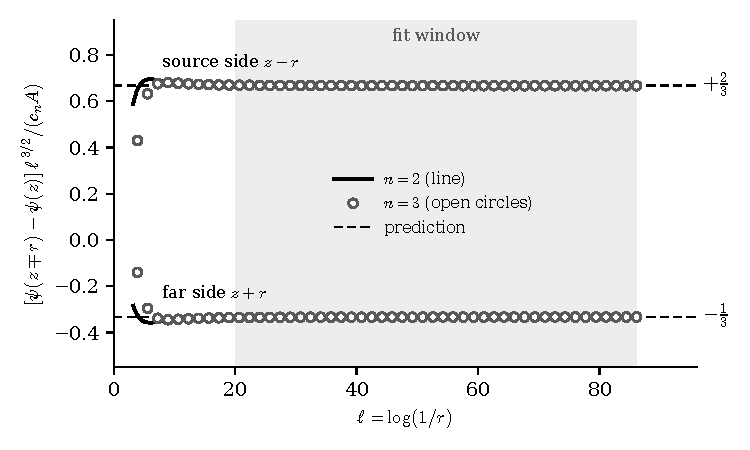
\includegraphics[width=0.8\textwidth]{numerics/fig_kink_split.pdf}
\caption{Generation-1 kink profile at $L=0.6$ (even ground state, $s=0$, $\lambda=-2.417$, $A=1.567$; P1, grading $\rho=1.15$ down to $r=10^{-40}$). Plotted: the one-sided excursions $[\psi(q\mp r)-\psi(q)]\ell^{3/2}/(c_nA)$ at $q=y_n=L-\log n$, with $\psi(q)$ from the cusp fit (the node value at $q$ itself is truncated). Dashed: the predicted split $+\frac23$ (source side) and $-\frac13$ (far side) of K3. Line: $n=2$; circles: $n=3$ (every 12th node). The two coincide because $D\approx-0.002$ and $\beta_2=\beta_3=0$ here, so the $O(1/\ell)$ correction nearly vanishes. Fitted limits: $0.66679$ and $-0.33335$ for both points. Data from the pre-registered run \texttt{k06\_r1.15.json}.}\label{fig:kink}
\end{figure}
 from papers/weil-edge/.
% Needs: booktabs, array, amsmath, graphicx. The tabulars tab_kink_*.tex, tab_k5.tex, tab_tail_*.tex are generated by
% make_tables.py from data; tab_detect.tex, tab_H.tex and tab_cX.tex are copied by hand from the sources in numerics.md.
% Statement labels follow the synthesis note: K1 (edge law to second order, D = lambda + log 2pi + gamma),
% K3 (first-order kink profile), K6 (jump-ratio offset with prime-power boosts), T2 (first-order tail law),
% T4 / Pred. F (lambda-shifted second-order tail law). Registered IDs of the pre-registration in brackets.

\begin{table}[p]\centering\footnotesize\setlength\tabcolsep{3pt}
% Which numerical checks can detect a wrong constant. Hand-written; every number is copied from the source named
% in numerics.md (section "Sources"), and none is new except the error bars of the kink rows (kink_errors.out).
\begin{tabular}{>{\raggedright\arraybackslash}p{3.6cm}>{\raggedright\arraybackslash}p{3.3cm}>{\raggedright\arraybackslash}p{3.9cm}>{\raggedright\arraybackslash}p{4.6cm}}
\toprule
Check & Statement tested & Result & Can it detect a wrong constant? \\
\midrule
\multicolumn{4}{l}{\emph{Edge law (E) and Hadamard formula (H)}}\\
Cross identity, nested and translated windows (N1, N2) & exact cross identity & rel.\ error $2\cdot10^{-8}$--$7.3\cdot10^{-8}$ & No: no edge trace appears in it \\
Edge-free identity $X^2/(\lambda_e'\lambda_o')$ (N3) & mixed identity, Thm.~3(e) & $0.99801$--$1.00064$ (4 cases) & No: both sides scale by $\kappa^2$ \\
Pure log, $L(\lambda_e-\lambda_o)\Phi'(0)$ (N4) & mixed identity and $A^2=\frac1{2L}$ jointly & $\pm1.00000$ to $\pm1.00061$ (9 pairs) & No: $\kappa$ cancels \\
Sector ratio $(A_o/A_e)^2$ vs.\ $\lambda_o'/\lambda_e'$ (N5) & ratio form of (H) & agreement within $0.5\%$ (4 cases) & No: $\kappa$ cancels \\
Explicit formula of Thm.~1(3) (N7) & $A_+=\int v_qf_q$ & matches edge fit to $(1$--$3)\cdot10^{-5}$ & Tests Thm.~1(3), not the constant of (H) \\
$-\lambda'/(2A^2)$, independent P0 code (13 cases) & (H) with constant 2 & within $3\cdot10^{-3}$ of 1 (base); within $6\cdot10^{-4}$ after refinement & \textbf{Yes}: a layer constant $\kappa$ would give ratio $\kappa$; $\kappa=1\pm3\cdot10^{-3}$ \\
$-\lambda'/(2A^2)$, project hp-FEM (N9) & same & $0.9987$--$1.0024$ (about $1\%$ model uncertainty) & \textbf{Yes}, at the $1\%$ level \\
$|\lambda'|/2A^2$, P1 tail states & same & $0.9960$--$1.0097$ (12 states) & \textbf{Yes}, at the $1\%$ level (edge grading $10^{-9}$ limits $A$) \\
$D_{\rm fit}-D$, $D=\lambda+\log2\pi+\gamma$ (K1) & second-order edge law & $+0.0013$ to $+0.0049$ (registered main meshes); $+0.0039$, $+0.0051$ in the $L=1.0$ rerun & \textbf{Yes} at $\pm0.005$; would see a missing $\gamma$ or $\log2\pi$ \\
\midrule
\multicolumn{4}{l}{\emph{Kink law}}\\
$\kappa_0$, generation 1 (K3, $k=1$) & jump coefficient $1$ & $0.9986$--$1.0019$; systematic error $\le0.002$ ($\le0.0043$ on the $L=1.0$ sensitivity mesh) & \textbf{Yes}, to about $0.2$--$0.4\%$ \\
$\sigma_0$, side ratio, generation 1 & split $\frac23:-\frac13$ & $\sigma_0=0.3322$--$0.3346$; side $-1.9969$ to $-2.0035$ & \textbf{Yes}: excludes a one-sided germ ($\sigma_0=1$) and an odd one ($\sigma_0=0$) \\
Generation 2 (K3, $k=2$) & $\frac35:-\frac25$, chain weight $W$ & $\kappa_0$ $0.991$--$1.005$; $\sigma_0$ $0.197$--$0.202$ & \textbf{Yes}, to about $1\%$ \\
Offset $1/\rho_n-\ell\to-D-\beta_n$ (K6) & $D$ and boosts $\beta_n$ & $|{\rm dev}|\le0.0025$ at $L=0.6,0.8$; $\le0.0020$ at $L=1.0$ in the rerun (registered meshes: FAIL) & \textbf{Yes}: boosts $0.347$, $0.693$ resolved to $\pm0.003$ \\
\midrule
\multicolumn{4}{l}{\emph{Tail law}}\\
$Z/P_1$, $\tau/\tau_{\rm pred}$ (T4 / Pred.~F) & $\lambda$-shifted second-order law & $Z/P_1=0.80$--$1.00$; $-8.7\%$ to $+0.03\%$ for $T\ge400$ & Coarsely: sees the $\lambda$-shift (factor $2$--$5$); blind to errors below about $10\%$ at $T\le10^4$ \\
Sector split, $X=8$ & coefficient $2c_X$ & $\alpha/(2c_8)=1.04$--$1.37$, $\sigma\approx0.13$ & \textbf{Yes}, at $\pm30\%$; $\alpha=0$ excluded by $7$--$11\sigma$ \\
Zero-side split, $X=2,3$ & $\pm c_X$ term with sector sign & with term $0.968$--$1.014$; without $0.86$--$0.91$ / $1.09$--$1.13$ & \textbf{Yes} for sign and size, at about $\pm30\%$ \\
Leading law $\pi TZ\to|\lambda'|$ (T2) & first-order law & $\tau(6400)=0.47$--$0.81$ & No: not testable at $T\le10^4$ for these $\lambda$ \\
\bottomrule
\end{tabular}

\caption{Which numerical checks can detect a wrong constant. The exact identities (N1--N5) hold for any value $\kappa$ of the layer constant in Lemmas~8.2--8.3, so they cannot confirm the constant $2$ in (H); only absolute determinations of $A$ compared with $\lambda'$ can. ``Yes'' gives the size of error the check would see. Nothing here is certified, and nothing here bears on the Riemann hypothesis.}\label{tab:detect}
\end{table}

\begin{table}[p]\centering\footnotesize\setlength\tabcolsep{3pt}
% Absolute checks of the constant 2 in (H): -lambda'/(2A^2) = 1, with A from an edge fit and lambda' from finite
% differences. Copied from note_v2 sec. 13.1 and note-v2/evidence.out (P0 code written during the final internal AI referee pass) and
% from [NUM] (P1). The P0 refinement column applies the measured h0-shift (see the source); it assumes smooth,
% additive mesh errors.
\begin{tabular}{>{\raggedright\arraybackslash}p{3.3cm}>{\raggedright\arraybackslash}p{1.3cm}>{\raggedright\arraybackslash}p{2.0cm}>{\raggedright\arraybackslash}p{3.7cm}>{\raggedright\arraybackslash}p{3.0cm}l}
\toprule
case & primes & states & base mesh & refined & code \\
\midrule
pure log, $L=0.5$ (companion paper) & none & $e_0$, $o_0$, $e_1$ & $2LA^2=1.00020$, $1.00043$, $1.00062$ & excess shrinks by $0.54$--$0.68$ per halving of $h_0$ & P0 \\
Weil, $L=0.3$ & none active & $s=0$ e/o, $s=1$ e/o & $0.99982$, $0.99958$, $0.99949$, $0.99959$ & --- & P0 \\
Weil, $L=0.4$, graded at $\pm(L-\log2)$ & $2$ & $s=0$ e/o, $s=1$ e/o & $0.99975$, $0.99876$, $0.99812$, $0.99887$ & $s=0$: $1.00020$, $1.00026$ & P0 \\
Weil, $L=0.6$, graded & $2,3$ & $s=0$ e/o & $0.99969$, $0.99724$ & $1.00007$, $0.99943$ & P0 \\
contrast: $L=0.4$, not graded at $L-\log2$ & $2$ & 4 states & $0.995$--$0.998$ & $0.9996$--$1.006$ & P0 \\
\midrule
Weil, $X=6,8,10$, 12 tail states & all $n<X$ & $s=-1,0,5,20$ & $0.9960$--$1.0097$ & --- & P1 \\
Weil, $L=0.36$--$0.7$ & as active & $k=0,1$, $s=0,1$ & $0.9987$--$1.0024$ & --- & hp-FEM \\
\bottomrule
\end{tabular}

\caption{Absolute checks of the constant in (H): $-\lambda'/(2A^2)$, predicted to be $1$. P0: the piecewise-constant Galerkin code of the final internal referee, independent of the project's hp-FEM; edge mesh down to $r=10^{-150}$, $A$ fitted on $\ell\in[30,345]$ and extrapolated in the grading ratio. ``Refined'' adds the measured shift from $h_0=L/500$ to $L/2000$ (contrast row: $h_0=L/1000$). The $L=0.6$ odd entry is the weakest ($\lambda'$ from one mesh while $\lambda_o$ moves by $2\%$ under refinement). Fitted amplitudes with active primes carry an extra resolution bias of $0.15$--$0.3\%$ unless the mesh is graded at $\pm(L-\log n)$ (contrast row). The pure-log case is treated in the companion paper; it is listed only because it is one of the absolute checks. hp-FEM N9 has one exception, the true even ground state at $L=0.7$ ($\lambda'=-3.5\cdot10^{-11}$, at the double-precision floor, ratio $0.9915$).}\label{tab:H}
\end{table}

\begin{table}[p]\centering\footnotesize\setlength\tabcolsep{2.5pt}
\begin{tabular}{lrlrrrlll}
\toprule
$L$ & $s$ & sector & $\lambda$ & $A$ & rows & $\kappa_0$ (1) & $\sigma_0$ ($\frac13$) & side ($-2$) \\
\midrule
0.6 & +0 & even & $-2.4170$ & $1.567$ & 6 & $1.0001\pm0.0002$ & $0.3334\pm0.0001$ & $-2.0003\pm0.0003$ \\
0.6 & +0 & odd & $+0.0031$ & $0.261$ & 6 & $[1.0014,1.0015]\pm0.0019$ & $0.3346\pm0.0016$ & $[-2.0035,-2.0034]\pm0.0047$ \\
0.6 & +5 & odd & $-0.2481$ & $0.728$ & 6 & $[1.0011,1.0012]\pm0.0013$ & $[0.3342,0.3343]\pm0.0012$ & $[-2.0025,-2.0024]\pm0.0034$ \\
0.6 & +5 & odd & $+0.0034$ & $0.291$ & 6 & $[1.0014,1.0015]\pm0.0018$ & $0.3346\pm0.0016$ & $[-2.0035,-2.0034]\pm0.0047$ \\
0.8 & +0 & even & $-3.3154$ & $1.425$ & 3 & $[1.0000,1.0001]\pm0.0002$ & $0.3334\pm0.0001$ & $-2.0003\pm0.0002$ \\
0.8 & +5 & odd & $-0.6567$ & $1.437$ & 3 & $[1.0013,1.0019]\pm0.0019$ & $[0.3342,0.3345]\pm0.0013$ & $[-2.0023,-2.0020]\pm0.0028$ \\
1.0 reg. & +0 & even & $-4.3060$ & $1.645$ & 5 & $[0.9986,0.9996]\pm0.0012$ & $[0.3322,0.3330]\pm0.0004$ & $[-1.9990,-1.9969]\pm0.0010$ \\
1.0 reg. & +5 & odd & $-1.3522$ & $1.379$ & 5 & $[1.0000,1.0010]\pm0.0011$ & $[0.3331,0.3340]\pm0.0011$ & $[-2.0016,-1.9989]\pm0.0038$ \\
1.0 sens. & +0 & even & $-4.3060$ & $1.645$ & 5 & $[0.9996,0.9999]\pm0.0016$ & $[0.3330,0.3332]\pm0.0006$ & $[-1.9993,-1.9990]\pm0.0010$ \\
1.0 sens. & +5 & odd & $-1.3522$ & $1.379$ & 5 & $[1.0009,1.0013]\pm0.0043$ & $[0.3340,0.3343]\pm0.0026$ & $[-2.0023,-2.0016]\pm0.0053$ \\
1.0 diag.$^\dagger$ & +0 & even & $-4.3060$ & $1.645$ & 5 & $[0.9993,0.9997]\pm0.0006$ & $[0.3328,0.3331]\pm0.0006$ & $[-1.9992,-1.9989]\pm0.0016$ \\
1.0 diag.$^\dagger$ & +5 & odd & $-1.3522$ & $1.379$ & 5 & $[1.0012,1.0016]\pm0.0021$ & $[0.3343,0.3344]\pm0.0013$ & $-2.0024\pm0.0029$ \\
1.0 rerun$^\ddagger$ & +0 & even & $-4.3060$ & $1.645$ & 5 & $[0.9995,0.9998]\pm0.0004$ & $[0.3329,0.3331]\pm0.0004$ & $[-1.9991,-1.9988]\pm0.0011$ \\
1.0 rerun$^\ddagger$ & +5 & odd & $-1.3522$ & $1.379$ & 5 & $[1.0008,1.0011]\pm0.0012$ & $[0.3340,0.3341]\pm0.0009$ & $-2.0016\pm0.0021$ \\
\bottomrule
\end{tabular}

\caption{Generation-1 kink constants (K3 with $k=1$; registered K1). Fits $\mathsf J\ell^{3/2}/(c_nA)=\kappa_0+\kappa_1/\ell+\kappa_2/\ell^2$ and $\psi(q-r)+\psi(q+r)=2\psi(q)+c_nA\ell^{-3/2}(\sigma_0+\dots)$ on $\ell\in[20,\ell_{\max}-6]$, finest grading; side $=(\kappa_0+\sigma_0)/(\sigma_0-\kappa_0)$. Predictions in the headers. ``rows'': chain points $y_n$, $n<X$ (at $L=0.6$ with mirrors). Brackets give the range over rows; $\pm$ is a systematic band, not a standard deviation: the spread over grading ratios plus the change when the fit window starts at $\ell=15$ or $25$ instead of $20$ (\texttt{kink\_errors.out}). Original registered verdict on every row: PASS (50/50 graded rows; tolerances $0.005$, $0.003$, $0.015$). $^\dagger$Post-registration diagnostic, all coupled generation-2 points graded; not a registered verdict. $^\ddagger$The new pre-registered rerun (Table~\ref{tab:k5}), primary meshes; PASS 10/10 under the same tolerances (also with $\rho=1.15$ added).}\label{tab:kink1}
\end{table}

\begin{table}[p]\centering\footnotesize\setlength\tabcolsep{3pt}
\begin{tabular}{llrrlrrlll}
\toprule
$L$ & point & $W$ & $s$ & sector & $A$ & rows & $\kappa_0$ (1) & $\sigma_0$ ($\frac15$) & side ($-\frac32$) \\
\midrule
0.6 & $L-\log\frac{3}{2}$ & $0.3109$ & +0 & even & $1.567$ & 3 & $1.0005\pm0.0006$ & $0.2002\pm0.0002$ & $-1.5002\pm0.0002$ \\
0.6 & $L-\log\frac{3}{2}$ & $0.3109$ & +0 & odd & $0.261$ & 3 & $[1.0049,1.0050]\pm0.0073$ & $0.2018\pm0.0027$ & $-1.5025\pm0.0037$ \\
0.6 & $L-\log\frac{3}{2}$ & $0.3109$ & +5 & odd & $0.728$ & 3 & $[1.0038,1.0039]\pm0.0037$ & $0.2013\pm0.0019$ & $-1.5016\pm0.0036$ \\
0.6 & $L-\log\frac{3}{2}$ & $0.3109$ & +5 & odd & $0.291$ & 3 & $[1.0049,1.0050]\pm0.0071$ & $0.2018\pm0.0027$ & $-1.5025\pm0.0039$ \\
0.8 & $L-\log\frac{3}{2}$ & $0.3109$ & +0 & even & $1.425$ & 1 & $1.0001\pm0.0002$ & $0.2001\pm0.0001$ & $-1.5003\pm0.0001$ \\
0.8 & $L-\log\frac{4}{3}$ & $0.2198$ & +0 & even & $1.425$ & 1 & $1.0003\pm0.0005$ & $0.2001\pm0.0001$ & $-1.5003\pm0.0001$ \\
0.8 & $L-\log\frac{3}{2}$ & $0.3109$ & +5 & odd & $1.437$ & 1 & $1.0041\pm0.0038$ & $0.2010\pm0.0013$ & $-1.5005\pm0.0016$ \\
0.8 & $L-\log\frac{4}{3}$ & $0.2198$ & +5 & odd & $1.437$ & 1 & $1.0054\pm0.0046$ & $0.2013\pm0.0017$ & $-1.5006\pm0.0023$ \\
1.0 reg. & $L-\log6$ & $0.6218$ & +0 & even & $1.645$ & 1 & $0.9912\pm0.0050$ & $0.1967\pm0.0013$ & $-1.4953\pm0.0046$ \\
1.0 reg. & $L-\log6$ & $0.6218$ & +5 & odd & $1.379$ & 1 & $0.9936\pm0.0053$ & $0.1968\pm0.0030$ & $-1.4940\pm0.0079$ \\
1.0 sens. & $L-\log6$ & $0.6218$ & +0 & even & $1.645$ & 1 & $1.0000\pm0.0033$ & $0.2001\pm0.0004$ & $-1.5004\pm0.0015$ \\
1.0 sens. & $L-\log6$ & $0.6218$ & +5 & odd & $1.379$ & 1 & $1.0044\pm0.0103$ & $0.2017\pm0.0027$ & $-1.5024\pm0.0022$ \\
1.0 diag.$^\dagger$ & $L-\log6$ & $0.6218$ & +0 & even & $1.645$ & 1 & $0.9987\pm0.0011$ & $0.1996\pm0.0005$ & $-1.4995\pm0.0010$ \\
1.0 diag.$^\dagger$ & $L-\log6$ & $0.6218$ & +5 & odd & $1.379$ & 1 & $1.0040\pm0.0051$ & $0.2009\pm0.0012$ & $-1.5003\pm0.0007$ \\
1.0 rerun$^\ddagger$ & $L-\log6$ & $0.6218$ & +0 & even & $1.645$ & 1 & $0.9989\pm0.0006$ & $0.1996\pm0.0004$ & $-1.4994\pm0.0008$ \\
1.0 rerun$^\ddagger$ & $L-\log6$ & $0.6218$ & +5 & odd & $1.379$ & 1 & $1.0028\pm0.0030$ & $0.2007\pm0.0009$ & $-1.5003\pm0.0010$ \\
\bottomrule
\end{tabular}

\caption{Generation-2 kink constants (K3 with $k=2$; registered K2): predicted jump coefficient $1$, cusp $\frac15$ and side ratio $-\frac32$, i.e.\ the split $\frac35:-\frac25$, with chain weight $W$ ($c_2c_3=0.3109$, $c_3c_4=0.2198$, $2c_2c_3=0.6218$). Same fits and error bands as Table~\ref{tab:kink1}. Original registered verdict: PASS 20/20 (tolerances $0.01$, $0.004$, $0.015$). $^\dagger$Post-registration diagnostic. $^\ddagger$New pre-registered rerun, primary meshes; PASS 2/2. In the rerun the generation-3 point $L-\log\frac65$, coupled to $L-\log6$, is also graded.}\label{tab:kink2}
\end{table}

\begin{table}[p]\centering\footnotesize\setlength\tabcolsep{3pt}
\begin{tabular}{llrrlll}
\toprule
$L$, mesh & state & $n$ & $\beta_n$ & $b_0+D+\beta_n$ & $\max_\rho|b_0+D_{\rm fit}+\beta_n|$ & verdict \\
\midrule
0.6 & $s=+0$ even, $\lambda=-2.417$ & 3 & $0.000$ & $-0.0005\pm0.0006$ & $0.0008$ & PASS \\
0.6 & $s=+0$ even, $\lambda=-2.417$ & 2 & $0.000$ & $-0.0005\pm0.0006$ & $0.0008$ & PASS \\
0.6 & $s=+0$ odd, $\lambda=+0.003$ & 3 & $0.000$ & $-0.0018\pm0.0028$ & $0.0008$ & PASS \\
0.6 & $s=+0$ odd, $\lambda=+0.003$ & 2 & $0.000$ & $-0.0018\pm0.0062$ & $0.0008$ & PASS \\
0.6 & $s=+5$ odd, $\lambda=-0.248$ & 3 & $0.000$ & $-0.0016\pm0.0027$ & $0.0008$ & PASS \\
0.6 & $s=+5$ odd, $\lambda=-0.248$ & 2 & $0.000$ & $-0.0015\pm0.0016$ & $0.0009$ & PASS \\
0.6 & $s=+5$ odd, $\lambda=+0.003$ & 3 & $0.000$ & $-0.0018\pm0.0029$ & $0.0008$ & PASS \\
0.6 & $s=+5$ odd, $\lambda=+0.003$ & 2 & $0.000$ & $-0.0018\pm0.0057$ & $0.0008$ & PASS \\
0.8 & $s=+0$ even, $\lambda=-3.315$ & 4 & $0.693$ & $-0.0007\pm0.0007$ & $0.0028$ & PASS \\
0.8 & $s=+0$ even, $\lambda=-3.315$ & 3 & $0.000$ & $-0.0005\pm0.0006$ & $0.0029$ & PASS \\
0.8 & $s=+0$ even, $\lambda=-3.315$ & 2 & $0.347$ & $-0.0006\pm0.0007$ & $0.0029$ & PASS \\
0.8 & $s=+5$ odd, $\lambda=-0.657$ & 4 & $0.693$ & $-0.0025\pm0.0032$ & $0.0025$ & PASS \\
0.8 & $s=+5$ odd, $\lambda=-0.657$ & 3 & $0.000$ & $-0.0021\pm0.0026$ & $0.0030$ & PASS \\
0.8 & $s=+5$ odd, $\lambda=-0.657$ & 2 & $0.347$ & $-0.0023\pm0.0028$ & $0.0028$ & PASS \\
1.0 reg. & $s=+0$ even, $\lambda=-4.306$ & 7 & $0.000$ & $+0.0596\pm0.0367$ & $0.0643$ & \textbf{FAIL} \\
1.0 reg. & $s=+0$ even, $\lambda=-4.306$ & 5 & $0.000$ & $+0.0355\pm0.0219$ & $0.0396$ & \textbf{FAIL} \\
1.0 reg. & $s=+0$ even, $\lambda=-4.306$ & 4 & $0.693$ & $+0.0183\pm0.0112$ & $0.0222$ & \textbf{FAIL} \\
1.0 reg. & $s=+0$ even, $\lambda=-4.306$ & 3 & $0.000$ & $+0.0111\pm0.0070$ & $0.0148$ & \textbf{FAIL} \\
1.0 reg. & $s=+0$ even, $\lambda=-4.306$ & 2 & $0.347$ & $-0.0003\pm0.0005$ & $0.0032$ & PASS \\
1.0 reg. & $s=+5$ odd, $\lambda=-1.352$ & 7 & $0.000$ & $+0.0609\pm0.0394$ & $0.0668$ & \textbf{FAIL} \\
1.0 reg. & $s=+5$ odd, $\lambda=-1.352$ & 5 & $0.000$ & $+0.0357\pm0.0233$ & $0.0411$ & \textbf{FAIL} \\
1.0 reg. & $s=+5$ odd, $\lambda=-1.352$ & 4 & $0.693$ & $+0.0176\pm0.0116$ & $0.0226$ & \textbf{FAIL} \\
1.0 reg. & $s=+5$ odd, $\lambda=-1.352$ & 3 & $0.000$ & $+0.0102\pm0.0071$ & $0.0151$ & \textbf{FAIL} \\
1.0 reg. & $s=+5$ odd, $\lambda=-1.352$ & 2 & $0.347$ & $-0.0017\pm0.0021$ & $0.0030$ & PASS \\
1.0 sens. & $s=+0$ even, $\lambda=-4.306$ & 7 & $0.000$ & $-0.0138\pm0.0349$ & $0.0057$ & \textbf{FAIL} \\
1.0 sens. & $s=+0$ even, $\lambda=-4.306$ & 5 & $0.000$ & $-0.0100\pm0.0212$ & $0.0019$ & \textbf{FAIL} \\
1.0 sens. & $s=+0$ even, $\lambda=-4.306$ & 4 & $0.693$ & $-0.0073\pm0.0108$ & $0.0009$ & \textbf{FAIL} \\
1.0 sens. & $s=+0$ even, $\lambda=-4.306$ & 3 & $0.000$ & $-0.0063\pm0.0073$ & $0.0018$ & \textbf{FAIL} \\
1.0 sens. & $s=+0$ even, $\lambda=-4.306$ & 2 & $0.347$ & $-0.0048\pm0.0010$ & $0.0034$ & PASS \\
1.0 sens. & $s=+5$ odd, $\lambda=-1.352$ & 7 & $0.000$ & $-0.0172\pm0.0444$ & $0.0078$ & \textbf{FAIL} \\
1.0 sens. & $s=+5$ odd, $\lambda=-1.352$ & 5 & $0.000$ & $-0.0125\pm0.0270$ & $0.0031$ & \textbf{FAIL} \\
1.0 sens. & $s=+5$ odd, $\lambda=-1.352$ & 4 & $0.693$ & $-0.0094\pm0.0143$ & $0.0000$ & \textbf{FAIL} \\
1.0 sens. & $s=+5$ odd, $\lambda=-1.352$ & 3 & $0.000$ & $-0.0081\pm0.0103$ & $0.0013$ & \textbf{FAIL} \\
1.0 sens. & $s=+5$ odd, $\lambda=-1.352$ & 2 & $0.347$ & $-0.0062\pm0.0028$ & $0.0032$ & \textbf{FAIL} \\
1.0 diag.$^\dagger$ & $s=+0$ even, $\lambda=-4.306$ & 7 & $0.000$ & $-0.0009\pm0.0004$ & $0.0033$ & n/a \\
1.0 diag.$^\dagger$ & $s=+0$ even, $\lambda=-4.306$ & 5 & $0.000$ & $-0.0008\pm0.0007$ & $0.0034$ & n/a \\
1.0 diag.$^\dagger$ & $s=+0$ even, $\lambda=-4.306$ & 4 & $0.693$ & $-0.0007\pm0.0008$ & $0.0035$ & n/a \\
1.0 diag.$^\dagger$ & $s=+0$ even, $\lambda=-4.306$ & 3 & $0.000$ & $-0.0007\pm0.0008$ & $0.0035$ & n/a \\
1.0 diag.$^\dagger$ & $s=+0$ even, $\lambda=-4.306$ & 2 & $0.347$ & $-0.0010\pm0.0010$ & $0.0033$ & n/a \\
1.0 diag.$^\dagger$ & $s=+5$ odd, $\lambda=-1.352$ & 7 & $0.000$ & $-0.0039\pm0.0059$ & $0.0032$ & n/a \\
1.0 diag.$^\dagger$ & $s=+5$ odd, $\lambda=-1.352$ & 5 & $0.000$ & $-0.0035\pm0.0039$ & $0.0034$ & n/a \\
1.0 diag.$^\dagger$ & $s=+5$ odd, $\lambda=-1.352$ & 4 & $0.693$ & $-0.0040\pm0.0036$ & $0.0032$ & n/a \\
1.0 diag.$^\dagger$ & $s=+5$ odd, $\lambda=-1.352$ & 3 & $0.000$ & $-0.0036\pm0.0039$ & $0.0034$ & n/a \\
1.0 diag.$^\dagger$ & $s=+5$ odd, $\lambda=-1.352$ & 2 & $0.347$ & $-0.0039\pm0.0041$ & $0.0032$ & n/a \\
1.0 rerun$^\ddagger$ & $s=+0$ even, $\lambda=-4.306$ & 7 & $0.000$ & $-0.0005\pm0.0003$ & $0.0034$ & PASS \\
1.0 rerun$^\ddagger$ & $s=+0$ even, $\lambda=-4.306$ & 5 & $0.000$ & $-0.0004\pm0.0004$ & $0.0035$ & PASS \\
1.0 rerun$^\ddagger$ & $s=+0$ even, $\lambda=-4.306$ & 4 & $0.693$ & $-0.0003\pm0.0004$ & $0.0035$ & PASS \\
1.0 rerun$^\ddagger$ & $s=+0$ even, $\lambda=-4.306$ & 3 & $0.000$ & $-0.0004\pm0.0004$ & $0.0035$ & PASS \\
1.0 rerun$^\ddagger$ & $s=+0$ even, $\lambda=-4.306$ & 2 & $0.347$ & $-0.0005\pm0.0005$ & $0.0034$ & PASS \\
1.0 rerun$^\ddagger$ & $s=+5$ odd, $\lambda=-1.352$ & 7 & $0.000$ & $-0.0019\pm0.0028$ & $0.0032$ & PASS \\
1.0 rerun$^\ddagger$ & $s=+5$ odd, $\lambda=-1.352$ & 5 & $0.000$ & $-0.0017\pm0.0020$ & $0.0034$ & PASS \\
1.0 rerun$^\ddagger$ & $s=+5$ odd, $\lambda=-1.352$ & 4 & $0.693$ & $-0.0019\pm0.0020$ & $0.0032$ & PASS \\
1.0 rerun$^\ddagger$ & $s=+5$ odd, $\lambda=-1.352$ & 3 & $0.000$ & $-0.0017\pm0.0020$ & $0.0034$ & PASS \\
1.0 rerun$^\ddagger$ & $s=+5$ odd, $\lambda=-1.352$ & 2 & $0.347$ & $-0.0019\pm0.0022$ & $0.0032$ & PASS \\
1.0 rerun, $\rho\to1.15^\ddagger$ & $s=+0$ even, $\lambda=-4.306$ & 7 & $0.000$ & $-0.0005\pm0.0003$ & $0.0034$ & PASS \\
1.0 rerun, $\rho\to1.15^\ddagger$ & $s=+0$ even, $\lambda=-4.306$ & 5 & $0.000$ & $-0.0004\pm0.0004$ & $0.0035$ & PASS \\
1.0 rerun, $\rho\to1.15^\ddagger$ & $s=+0$ even, $\lambda=-4.306$ & 4 & $0.693$ & $-0.0004\pm0.0005$ & $0.0035$ & PASS \\
1.0 rerun, $\rho\to1.15^\ddagger$ & $s=+0$ even, $\lambda=-4.306$ & 3 & $0.000$ & $-0.0004\pm0.0004$ & $0.0035$ & PASS \\
1.0 rerun, $\rho\to1.15^\ddagger$ & $s=+0$ even, $\lambda=-4.306$ & 2 & $0.347$ & $-0.0005\pm0.0006$ & $0.0034$ & PASS \\
1.0 rerun, $\rho\to1.15^\ddagger$ & $s=+5$ odd, $\lambda=-1.352$ & 7 & $0.000$ & $-0.0019\pm0.0028$ & $0.0032$ & PASS \\
1.0 rerun, $\rho\to1.15^\ddagger$ & $s=+5$ odd, $\lambda=-1.352$ & 5 & $0.000$ & $-0.0017\pm0.0020$ & $0.0034$ & PASS \\
1.0 rerun, $\rho\to1.15^\ddagger$ & $s=+5$ odd, $\lambda=-1.352$ & 4 & $0.693$ & $-0.0019\pm0.0020$ & $0.0032$ & PASS \\
1.0 rerun, $\rho\to1.15^\ddagger$ & $s=+5$ odd, $\lambda=-1.352$ & 3 & $0.000$ & $-0.0018\pm0.0020$ & $0.0034$ & PASS \\
1.0 rerun, $\rho\to1.15^\ddagger$ & $s=+5$ odd, $\lambda=-1.352$ & 2 & $0.347$ & $-0.0019\pm0.0022$ & $0.0032$ & PASS \\
\bottomrule
\end{tabular}

\caption{Jump-ratio offset (K6; registered K5). Prediction: $1/\rho_n-\ell\to-D-\beta_n$, with $\rho_n=\mathsf J/(c_n\psi(L-r))$, $D=\lambda+\log2\pi+\gamma$ and boosts $\beta_n=W_2^+(y_n)/c_n$; at $L=0.6$ the prime power $4$ is not active, so every boost vanishes there. Registered pass rule (tolerance $0.005$): the grading-extrapolated $b_0+D+\beta_n$ \emph{and} the calibration-free $|b_0+D_{\rm fit}+\beta_n|$ at every grading. $\pm$: fit-window band plus, where three gradings exist, the spread of the two two-mesh extrapolations; with two gradings the extrapolation has no internal check. ``reg.'': the registered $L=1.0$ mesh, generation-2 points graded only to $10^{-16}$ ($\ell=36.8$, inside the fit window $[20,63]$). ``sens.'': the registered sensitivity mesh, one grading only (raw value, no extrapolation). These two meshes give the registered FAIL on 17 of the 20 graded $L=1.0$ rows; it stays in the record. $^\dagger$Post-registration diagnostic; its second mesh had a shorter fit window, so the calibrated column shows the $\rho=1.5$ value and no verdict is given. $^\ddagger$New pre-registered rerun (\texttt{PREREG\_K5\_L1.md}): every chain point coupled to a measured point graded through the whole fit window; primary verdict on $\rho\in\{1.5,1.25\}$, supplementary with $\rho=1.15$ added.}\label{tab:k5}
\end{table}

\begin{table}[p]\centering\footnotesize\setlength\tabcolsep{3pt}
\begin{tabular}{llrll}
\toprule
$L$, mesh & state & $D$ & $D_{\rm fit}-D$ & verdict \\
\midrule
0.6 & $s=+0$ even, $\lambda=-2.417$ & $-0.0019$ & $+0.0013\pm0.0008$ & PASS \\
0.6 & $s=+0$ odd, $\lambda=+0.003$ & $+2.4182$ & $+0.0025\pm0.0015$ & PASS \\
0.6 & $s=+5$ odd, $\lambda=-0.248$ & $+2.1670$ & $+0.0023\pm0.0011$ & PASS \\
0.6 & $s=+5$ odd, $\lambda=+0.003$ & $+2.4185$ & $+0.0025\pm0.0015$ & PASS \\
0.8 & $s=+0$ even, $\lambda=-3.315$ & $-0.9003$ & $+0.0033\pm0.0037$ & PASS \\
0.8 & $s=+5$ odd, $\lambda=-0.657$ & $+1.7584$ & $+0.0049\pm0.0029$ & PASS \\
1.0 reg. & $s=+0$ even, $\lambda=-4.306$ & $-1.8910$ & $+0.0035\pm0.0031$ & PASS \\
1.0 reg. & $s=+5$ odd, $\lambda=-1.352$ & $+1.0629$ & $+0.0047\pm0.0025$ & PASS \\
1.0 sens. & $s=+0$ even, $\lambda=-4.306$ & $-1.8910$ & $+0.0081\pm0.0033$ & \textbf{FAIL} \\
1.0 sens. & $s=+5$ odd, $\lambda=-1.352$ & $+1.0629$ & $+0.0094\pm0.0026$ & \textbf{FAIL} \\
1.0 diag.$^\dagger$ & $s=+0$ even, $\lambda=-4.306$ & $-1.8910$ & --- & n/a \\
1.0 diag.$^\dagger$ & $s=+5$ odd, $\lambda=-1.352$ & $+1.0629$ & --- & n/a \\
1.0 rerun$^\ddagger$ & $s=+0$ even, $\lambda=-4.306$ & $-1.8910$ & $+0.0039\pm0.0033$ & PASS \\
1.0 rerun$^\ddagger$ & $s=+5$ odd, $\lambda=-1.352$ & $+1.0629$ & $+0.0051\pm0.0027$ & \textbf{FAIL} \\
1.0 rerun, $\rho\to1.15^\ddagger$ & $s=+0$ even, $\lambda=-4.306$ & $-1.8910$ & $+0.0037\pm0.0036$ & PASS \\
1.0 rerun, $\rho\to1.15^\ddagger$ & $s=+5$ odd, $\lambda=-1.352$ & $+1.0629$ & $+0.005005\pm0.0029$ & \textbf{FAIL} \\
\bottomrule
\end{tabular}

\caption{Edge law to second order (K1; registered K0$'$): $\psi(L-r)=A(\ell-D)^{-1/2}+O(\ell^{-5/2})$, $D=\lambda+\log2\pi+\gamma$. $D_{\rm fit}=-a_1/a_0$ from $\psi(L-r)^{-2}=a_0\ell+a_1+a_2/\ell+a_3/\ell^2$ on $\ell\in[20,\ell_{\max}-6]$, extrapolated in the grading ratio; tolerance $0.005$. The deviation is positive in every row, so a small systematic offset of the fit model (up to about $0.005$) cannot be excluded; it is of the size of the fit-window band. In the new rerun the odd $s=5$ state fails this registered test by $1\cdot10^{-4}$ (primary) and $5\cdot10^{-6}$ (supplementary), well inside its band $\pm0.003$; it passed ($+0.0047$) on the registered mesh. Labels as in Table~\ref{tab:k5}.}\label{tab:k0}
\end{table}

\begin{table}[p]\centering\scriptsize\setlength\tabcolsep{2.5pt}
\begin{tabular}{rlrrrrrrrlll}
\toprule
$X$ & state & $\lambda$ & $|\lambda'|/2A^2$ & mesh & $[100,200]$ & $[400,800]$ & $[1600,3200]$ & $[6400,10300]$ & $\tau/\tau_{\rm pred}-1$, $T\ge400$ & no $\lambda$-shift & T1 \\
\midrule
6 & E0 & $-3.803$ & $0.9960$ & $2\cdot10^{-4}$ & $0.981$ & $0.995$ & $0.997$ & $1.000$ & $-0.003$ to $+0.001$ & $0.44\to0.65$ & PASS \\
6 & Em1 & $-7.632$ & $0.9979$ & $9\cdot10^{-5}$ & $0.975$ & $0.994$ & $0.993$ & $0.997$ & $-0.006$ to $-0.003$ & $0.28\to0.48$ & PASS \\
6 & O5 & $-0.920$ & $1.0097$ & $9\cdot10^{-4}$ & $0.869$ & $0.944$ & $0.972$ & $0.980$ & $-0.045$ to $-0.019$ & $0.67\to0.87$ & not graded \\
6 & O20 & $-4.590$ & $1.0040$ & $2\cdot10^{-4}$ & $0.886$ & $0.934$ & $0.967$ & $0.977$ & $-0.052$ to $-0.020$ & $0.35\to0.59$ & PASS \\
8 & E0 & $-4.515$ & $0.9983$ & $1\cdot10^{-4}$ & $0.951$ & $0.959$ & $0.982$ & $0.990$ & $-0.030$ to $-0.008$ & $0.42\to0.63$ & PASS \\
8 & Em1 & $-9.063$ & $0.9992$ & $5\cdot10^{-5}$ & $0.963$ & $0.962$ & $0.982$ & $0.988$ & $-0.028$ to $-0.011$ & $0.26\to0.45$ & PASS \\
8 & O5 & $-1.523$ & $1.0050$ & $7\cdot10^{-4}$ & $0.821$ & $0.938$ & $0.969$ & $0.980$ & $-0.047$ to $-0.017$ & $0.50\to0.78$ & PASS \\
8 & O20 & $-7.409$ & $1.0016$ & $5\cdot10^{-5}$ & $0.869$ & $0.944$ & $0.964$ & $0.975$ & $-0.046$ to $-0.021$ & $0.23\to0.46$ & PASS \\
10 & E0 & $-5.119$ & $0.9964$ & $2\cdot10^{-4}$ & $0.934$ & $0.966$ & $0.985$ & $0.993$ & $-0.025$ to $-0.006$ & $0.35\to0.58$ & PASS \\
10 & Em1 & $-10.263$ & $0.9984$ & $8\cdot10^{-5}$ & $0.954$ & $0.972$ & $0.984$ & $0.990$ & $-0.023$ to $-0.009$ & $0.22\to0.41$ & PASS \\
10 & O5 & $-2.097$ & $1.0085$ & $1\cdot10^{-3}$ & $0.796$ & $0.913$ & $0.954$ & $0.968$ & $-0.069$ to $-0.027$ & $0.47\to0.75$ & PASS \\
10 & O20 & $-10.205$ & $1.0021$ & $1\cdot10^{-4}$ & $0.888$ & $0.932$ & $0.959$ & $0.971$ & $-0.054$ to $-0.026$ & $0.21\to0.40$ & PASS \\
\bottomrule
\end{tabular}

\caption{Tail law, second order (T4 / Pred.~F; registered T1, T1-full, T1-$\lambda$) on actual zeta zeros ($\gamma\le10\,303$, Arb). Columns: $Z/P_1$ on four of the seven blocks, where $Z$ is the zero-side block sum and $P_1=(|\lambda'|/\pi)\int(a+\varepsilon c_X)/(t^2(a-\lambda))$; the range of $\tau/\tau_{\rm pred}-1$ for $T\ge400$; and $Z/P$ without the $\lambda$-shift, first to last block. ``mesh'': largest fine-versus-base block difference (the numerical error of $Z$). The deviations from $1$ are not numerical error: they are the unmodelled $O(a^{-2})$ remainder, always negative, of the order of $\sum_{n<X}c_n^2/a^2$. The registered tolerance was generous ($0.13$--$0.21$ on $[400,800]$); every graded state passed inside it by at least a factor $2$. States: ground states of their sector at pole strength $s$ (E0: $s=0$, Em1: $s=-1$, O5: $s=5$, O20: $s=20$); large $|\lambda|$, so these test the theorems where $\lambda/\log T$ is large, not the true $s=1$ form at small $\lambda$.}\label{tab:T1}
\end{table}

\begin{table}[p]\centering\footnotesize\setlength\tabcolsep{3pt}
\begin{tabular}{rrllrrl}
\toprule
$X$ & $2c_X$ & pair & $\alpha\pm\sigma_\alpha$ & $\beta$ & $(\alpha-2c_X)/\sigma_\alpha$ & verdict \\
\midrule
6 & $0.000$ & (E0,O20) & $+0.018\pm0.072$ & $+1.38$ & $+0.3$ & PASS \\
6 & $0.000$ & (Em1,O20) & $+0.012\pm0.068$ & $+1.65$ & $+0.2$ & PASS \\
8 & $0.490$ & (E0,O5) & $+0.512\pm0.067$ & $+1.89$ & $+0.3$ & PASS \\
8 & $0.490$ & (E0,O20) & $+0.658\pm0.064$ & $-0.67$ & $+2.6$ & PASS \\
8 & $0.490$ & (Em1,O5) & $+0.525\pm0.063$ & $+2.36$ & $+0.6$ & PASS \\
8 & $0.490$ & (Em1,O20) & $+0.671\pm0.061$ & $-0.20$ & $+3.0$ & PASS \\
10 & $0.000$ & (E0,O5) & $+0.323\pm0.178$ & $+1.14$ & $+1.8$ & PASS \\
10 & $0.000$ & (E0,O20) & $+0.430\pm0.183$ & $-1.89$ & $+2.4$ & PASS \\
10 & $0.000$ & (Em1,O5) & $+0.331\pm0.186$ & $+1.61$ & $+1.8$ & PASS \\
10 & $0.000$ & (Em1,O20) & $+0.438\pm0.191$ & $-1.43$ & $+2.3$ & PASS \\
\bottomrule
\end{tabular}

\caption{Sector split (registered T2): fit of $S_k=\ln(Z_e/E_e)_k-\ln(Z_o/E_o)_k=\alpha\langle1/a\rangle_k+\beta\langle a^{-2}\rangle_k$ over six blocks; prediction $\alpha=2c_X$. Registered pass rule $|\alpha-2c_X|\le\max(0.10,3\sigma_\alpha)$. At $X=8$ two pairs are $2.6\sigma$ and $3.0\sigma$ high; the second passes the $3\sigma$ rule by less than $0.003$. The $X=10$ control lies between $0$ and $2c_8$ and does not discriminate. At $T\le10^4$ the $1/a$ split cannot be separated cleanly from the $a^{-2}$ kink terms.}\label{tab:T2}
\end{table}

\begin{table}[p]\centering\footnotesize\setlength\tabcolsep{3pt}
% The c_X term at prime-power X = e^{2L}: zero-side tests on actual zeta zeros, with controls.
% Ratios are measured zero-side block sums over the prediction with (P_F, P_1) and without (P_noX, P_0) the c_X term.
% Ranges are over the blocks listed; they are the honest spread (no fitted error model). Sources in numerics.md.
\begin{tabular}{>{\raggedright\arraybackslash}p{2.1cm}>{\raggedright\arraybackslash}p{2.1cm}>{\raggedright\arraybackslash}p{2.3cm}>{\raggedright\arraybackslash}p{2.2cm}>{\raggedright\arraybackslash}p{4.4cm}>{\raggedright\arraybackslash}p{1.9cm}}
\toprule
$X$ ($c_X$) & state & code, zeros & blocks & with $c_X$ term & without \\
\midrule
$2$ ($0.490$) & $s=1$ even & P0, $\gamma_1$--$\gamma_{1500}$ & $[250,1981]$, 3 blocks & $0.988$--$1.003$ & $1.092$--$1.105$ \\
 & $s=1$ odd & & & $0.998$--$1.008$ & $0.887$--$0.909$ \\
 & $s=0$ even & & & $0.977$--$0.997$ & $1.086$--$1.096$ \\
 & $s=0$ odd & & & $0.998$--$1.009$ & $0.887$--$0.910$ \\
$3$ ($0.634$) & $s=0$ even & P0, $\gamma_1$--$\gamma_{1500}$ & $[250,1981]$, 3 blocks & $0.968$--$0.995$ & $1.106$--$1.127$ \\
 & $s=0$ odd & & & $0.999$--$1.014$ & $0.859$--$0.891$ \\
control $L=0.4$ ($0$) & $s=0$ even / odd & P0, $\gamma_1$--$\gamma_{1500}$ & $[250,1981]$, 3 blocks & $0.971$--$0.992$ / $0.996$--$0.999$ & (same) \\
\midrule
$4$ ($0.347$) & $s=0$ even & P0, $\gamma\le1980$ & $[100,1600]$, 4 blocks & $0.989$--$0.994$ ($h_0=L/1000$); $0.991$--$0.993$ ($L/2000$) & $1.060$--$1.104$ \\
\midrule
$8$ ($0.245$) & 4 even/odd pairs & P1, pre-reg., $\gamma\le10\,303$ & 6 blocks, $T_1\ge200$ & split $\alpha=0.512$--$0.671$, $\sigma_\alpha=0.061$--$0.067$ (prediction $2c_8=0.490$) & --- \\
control $6$ ($0$) & 2 pairs & P1, pre-reg. & same & $\alpha=+0.018\pm0.072$, $+0.012\pm0.068$ & --- \\
control $10$ ($0$) & 4 pairs & P1, pre-reg. & same & $\alpha=0.32$--$0.44$, $\sigma_\alpha=0.18$--$0.19$ (uninformative) & --- \\
$8$ vs.\ $6,10$ (post hoc) & even / odd & P1, pre-reg. & $[400,10300]$ & $Z/P_0$ offset $\approx+0.03$ / $-0.03$ at $T\approx4000$ (prediction $\pm c_8\langle1/a\rangle=\pm0.037$) & --- \\
\bottomrule
\end{tabular}

\caption{The $\pm c_X$ term at prime-power $X=e^{2L}$, on actual zeros. $X=2,3$: no $nm=X$ competition, the cleanest test (P0 eigenfunctions, $-\lambda'/2A^2=0.995$--$0.999$). $X=4$: even sector only; the odd state there has $|A|\sim0.02$ and $\lambda_o$ is not mesh-converged, and the derivative-free split matches $2c_4\langle1/a\rangle$ only within $10$--$30\%$. $X=8$: pre-registered (Table~\ref{tab:T2}). The post-hoc row compares $Z/P_0$ across $X$ for states of the same kind; the states differ in $\lambda$. The $c_X$ term is supported at $X=2,3,4,8$; at $X=8$ it is not cleanly separated from the $\ell^{-2}$ kink terms.}\label{tab:cX}
\end{table}

\begin{figure}[p]\centering
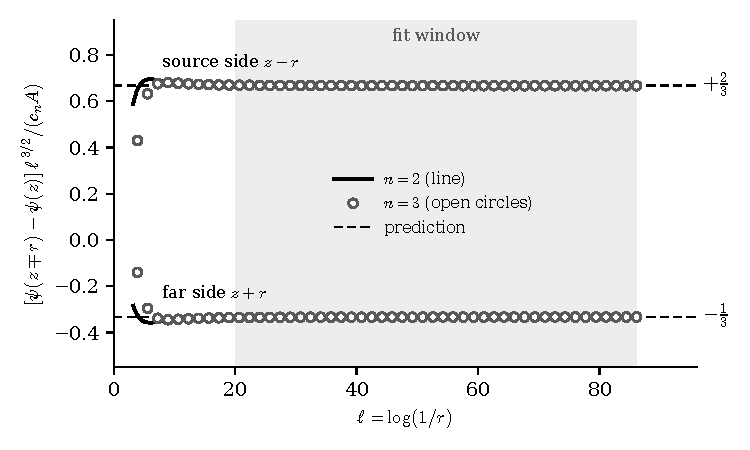
\includegraphics[width=0.8\textwidth]{numerics/fig_kink_split.pdf}
\caption{Generation-1 kink profile at $L=0.6$ (even ground state, $s=0$, $\lambda=-2.417$, $A=1.567$; P1, grading $\rho=1.15$ down to $r=10^{-40}$). Plotted: the one-sided excursions $[\psi(q\mp r)-\psi(q)]\ell^{3/2}/(c_nA)$ at $q=y_n=L-\log n$, with $\psi(q)$ from the cusp fit (the node value at $q$ itself is truncated). Dashed: the predicted split $+\frac23$ (source side) and $-\frac13$ (far side) of K3. Line: $n=2$; circles: $n=3$ (every 12th node). The two coincide because $D\approx-0.002$ and $\beta_2=\beta_3=0$ here, so the $O(1/\ell)$ correction nearly vanishes. Fitted limits: $0.66679$ and $-0.33335$ for both points. Data from the pre-registered run \texttt{k06\_r1.15.json}.}\label{fig:kink}
\end{figure}
 from papers/weil-edge/.
% Needs: booktabs, array, amsmath, graphicx. The tabulars tab_kink_*.tex, tab_k5.tex, tab_tail_*.tex are generated by
% make_tables.py from data; tab_detect.tex, tab_H.tex and tab_cX.tex are copied by hand from the sources in numerics.md.
% Statement labels follow the synthesis note: K1 (edge law to second order, D = lambda + log 2pi + gamma),
% K3 (first-order kink profile), K6 (jump-ratio offset with prime-power boosts), T2 (first-order tail law),
% T4 / Pred. F (lambda-shifted second-order tail law). Registered IDs of the pre-registration in brackets.

\begin{table}[p]\centering\footnotesize\setlength\tabcolsep{3pt}
% Which numerical checks can detect a wrong constant. Hand-written; every number is copied from the source named
% in numerics.md (section "Sources"), and none is new except the error bars of the kink rows (kink_errors.out).
\begin{tabular}{>{\raggedright\arraybackslash}p{3.6cm}>{\raggedright\arraybackslash}p{3.3cm}>{\raggedright\arraybackslash}p{3.9cm}>{\raggedright\arraybackslash}p{4.6cm}}
\toprule
Check & Statement tested & Result & Can it detect a wrong constant? \\
\midrule
\multicolumn{4}{l}{\emph{Edge law (E) and Hadamard formula (H)}}\\
Cross identity, nested and translated windows (N1, N2) & exact cross identity & rel.\ error $2\cdot10^{-8}$--$7.3\cdot10^{-8}$ & No: no edge trace appears in it \\
Edge-free identity $X^2/(\lambda_e'\lambda_o')$ (N3) & mixed identity, Thm.~3(e) & $0.99801$--$1.00064$ (4 cases) & No: both sides scale by $\kappa^2$ \\
Pure log, $L(\lambda_e-\lambda_o)\Phi'(0)$ (N4) & mixed identity and $A^2=\frac1{2L}$ jointly & $\pm1.00000$ to $\pm1.00061$ (9 pairs) & No: $\kappa$ cancels \\
Sector ratio $(A_o/A_e)^2$ vs.\ $\lambda_o'/\lambda_e'$ (N5) & ratio form of (H) & agreement within $0.5\%$ (4 cases) & No: $\kappa$ cancels \\
Explicit formula of Thm.~1(3) (N7) & $A_+=\int v_qf_q$ & matches edge fit to $(1$--$3)\cdot10^{-5}$ & Tests Thm.~1(3), not the constant of (H) \\
$-\lambda'/(2A^2)$, independent P0 code (13 cases) & (H) with constant 2 & within $3\cdot10^{-3}$ of 1 (base); within $6\cdot10^{-4}$ after refinement & \textbf{Yes}: a layer constant $\kappa$ would give ratio $\kappa$; $\kappa=1\pm3\cdot10^{-3}$ \\
$-\lambda'/(2A^2)$, project hp-FEM (N9) & same & $0.9987$--$1.0024$ (about $1\%$ model uncertainty) & \textbf{Yes}, at the $1\%$ level \\
$|\lambda'|/2A^2$, P1 tail states & same & $0.9960$--$1.0097$ (12 states) & \textbf{Yes}, at the $1\%$ level (edge grading $10^{-9}$ limits $A$) \\
$D_{\rm fit}-D$, $D=\lambda+\log2\pi+\gamma$ (K1) & second-order edge law & $+0.0013$ to $+0.0049$ (registered main meshes); $+0.0039$, $+0.0051$ in the $L=1.0$ rerun & \textbf{Yes} at $\pm0.005$; would see a missing $\gamma$ or $\log2\pi$ \\
\midrule
\multicolumn{4}{l}{\emph{Kink law}}\\
$\kappa_0$, generation 1 (K3, $k=1$) & jump coefficient $1$ & $0.9986$--$1.0019$; systematic error $\le0.002$ ($\le0.0043$ on the $L=1.0$ sensitivity mesh) & \textbf{Yes}, to about $0.2$--$0.4\%$ \\
$\sigma_0$, side ratio, generation 1 & split $\frac23:-\frac13$ & $\sigma_0=0.3322$--$0.3346$; side $-1.9969$ to $-2.0035$ & \textbf{Yes}: excludes a one-sided germ ($\sigma_0=1$) and an odd one ($\sigma_0=0$) \\
Generation 2 (K3, $k=2$) & $\frac35:-\frac25$, chain weight $W$ & $\kappa_0$ $0.991$--$1.005$; $\sigma_0$ $0.197$--$0.202$ & \textbf{Yes}, to about $1\%$ \\
Offset $1/\rho_n-\ell\to-D-\beta_n$ (K6) & $D$ and boosts $\beta_n$ & $|{\rm dev}|\le0.0025$ at $L=0.6,0.8$; $\le0.0020$ at $L=1.0$ in the rerun (registered meshes: FAIL) & \textbf{Yes}: boosts $0.347$, $0.693$ resolved to $\pm0.003$ \\
\midrule
\multicolumn{4}{l}{\emph{Tail law}}\\
$Z/P_1$, $\tau/\tau_{\rm pred}$ (T4 / Pred.~F) & $\lambda$-shifted second-order law & $Z/P_1=0.80$--$1.00$; $-8.7\%$ to $+0.03\%$ for $T\ge400$ & Coarsely: sees the $\lambda$-shift (factor $2$--$5$); blind to errors below about $10\%$ at $T\le10^4$ \\
Sector split, $X=8$ & coefficient $2c_X$ & $\alpha/(2c_8)=1.04$--$1.37$, $\sigma\approx0.13$ & \textbf{Yes}, at $\pm30\%$; $\alpha=0$ excluded by $7$--$11\sigma$ \\
Zero-side split, $X=2,3$ & $\pm c_X$ term with sector sign & with term $0.968$--$1.014$; without $0.86$--$0.91$ / $1.09$--$1.13$ & \textbf{Yes} for sign and size, at about $\pm30\%$ \\
Leading law $\pi TZ\to|\lambda'|$ (T2) & first-order law & $\tau(6400)=0.47$--$0.81$ & No: not testable at $T\le10^4$ for these $\lambda$ \\
\bottomrule
\end{tabular}

\caption{Which numerical checks can detect a wrong constant. The exact identities (N1--N5) hold for any value $\kappa$ of the layer constant in Lemmas~8.2--8.3, so they cannot confirm the constant $2$ in (H); only absolute determinations of $A$ compared with $\lambda'$ can. ``Yes'' gives the size of error the check would see. Nothing here is certified, and nothing here bears on the Riemann hypothesis.}\label{tab:detect}
\end{table}

\begin{table}[p]\centering\footnotesize\setlength\tabcolsep{3pt}
% Absolute checks of the constant 2 in (H): -lambda'/(2A^2) = 1, with A from an edge fit and lambda' from finite
% differences. Copied from note_v2 sec. 13.1 and note-v2/evidence.out (P0 code written during the final internal AI referee pass) and
% from [NUM] (P1). The P0 refinement column applies the measured h0-shift (see the source); it assumes smooth,
% additive mesh errors.
\begin{tabular}{>{\raggedright\arraybackslash}p{3.3cm}>{\raggedright\arraybackslash}p{1.3cm}>{\raggedright\arraybackslash}p{2.0cm}>{\raggedright\arraybackslash}p{3.7cm}>{\raggedright\arraybackslash}p{3.0cm}l}
\toprule
case & primes & states & base mesh & refined & code \\
\midrule
pure log, $L=0.5$ (companion paper) & none & $e_0$, $o_0$, $e_1$ & $2LA^2=1.00020$, $1.00043$, $1.00062$ & excess shrinks by $0.54$--$0.68$ per halving of $h_0$ & P0 \\
Weil, $L=0.3$ & none active & $s=0$ e/o, $s=1$ e/o & $0.99982$, $0.99958$, $0.99949$, $0.99959$ & --- & P0 \\
Weil, $L=0.4$, graded at $\pm(L-\log2)$ & $2$ & $s=0$ e/o, $s=1$ e/o & $0.99975$, $0.99876$, $0.99812$, $0.99887$ & $s=0$: $1.00020$, $1.00026$ & P0 \\
Weil, $L=0.6$, graded & $2,3$ & $s=0$ e/o & $0.99969$, $0.99724$ & $1.00007$, $0.99943$ & P0 \\
contrast: $L=0.4$, not graded at $L-\log2$ & $2$ & 4 states & $0.995$--$0.998$ & $0.9996$--$1.006$ & P0 \\
\midrule
Weil, $X=6,8,10$, 12 tail states & all $n<X$ & $s=-1,0,5,20$ & $0.9960$--$1.0097$ & --- & P1 \\
Weil, $L=0.36$--$0.7$ & as active & $k=0,1$, $s=0,1$ & $0.9987$--$1.0024$ & --- & hp-FEM \\
\bottomrule
\end{tabular}

\caption{Absolute checks of the constant in (H): $-\lambda'/(2A^2)$, predicted to be $1$. P0: the piecewise-constant Galerkin code of the final internal referee, independent of the project's hp-FEM; edge mesh down to $r=10^{-150}$, $A$ fitted on $\ell\in[30,345]$ and extrapolated in the grading ratio. ``Refined'' adds the measured shift from $h_0=L/500$ to $L/2000$ (contrast row: $h_0=L/1000$). The $L=0.6$ odd entry is the weakest ($\lambda'$ from one mesh while $\lambda_o$ moves by $2\%$ under refinement). Fitted amplitudes with active primes carry an extra resolution bias of $0.15$--$0.3\%$ unless the mesh is graded at $\pm(L-\log n)$ (contrast row). The pure-log case is treated in the companion paper; it is listed only because it is one of the absolute checks. hp-FEM N9 has one exception, the true even ground state at $L=0.7$ ($\lambda'=-3.5\cdot10^{-11}$, at the double-precision floor, ratio $0.9915$).}\label{tab:H}
\end{table}

\begin{table}[p]\centering\footnotesize\setlength\tabcolsep{2.5pt}
\begin{tabular}{lrlrrrlll}
\toprule
$L$ & $s$ & sector & $\lambda$ & $A$ & rows & $\kappa_0$ (1) & $\sigma_0$ ($\frac13$) & side ($-2$) \\
\midrule
0.6 & +0 & even & $-2.4170$ & $1.567$ & 6 & $1.0001\pm0.0002$ & $0.3334\pm0.0001$ & $-2.0003\pm0.0003$ \\
0.6 & +0 & odd & $+0.0031$ & $0.261$ & 6 & $[1.0014,1.0015]\pm0.0019$ & $0.3346\pm0.0016$ & $[-2.0035,-2.0034]\pm0.0047$ \\
0.6 & +5 & odd & $-0.2481$ & $0.728$ & 6 & $[1.0011,1.0012]\pm0.0013$ & $[0.3342,0.3343]\pm0.0012$ & $[-2.0025,-2.0024]\pm0.0034$ \\
0.6 & +5 & odd & $+0.0034$ & $0.291$ & 6 & $[1.0014,1.0015]\pm0.0018$ & $0.3346\pm0.0016$ & $[-2.0035,-2.0034]\pm0.0047$ \\
0.8 & +0 & even & $-3.3154$ & $1.425$ & 3 & $[1.0000,1.0001]\pm0.0002$ & $0.3334\pm0.0001$ & $-2.0003\pm0.0002$ \\
0.8 & +5 & odd & $-0.6567$ & $1.437$ & 3 & $[1.0013,1.0019]\pm0.0019$ & $[0.3342,0.3345]\pm0.0013$ & $[-2.0023,-2.0020]\pm0.0028$ \\
1.0 reg. & +0 & even & $-4.3060$ & $1.645$ & 5 & $[0.9986,0.9996]\pm0.0012$ & $[0.3322,0.3330]\pm0.0004$ & $[-1.9990,-1.9969]\pm0.0010$ \\
1.0 reg. & +5 & odd & $-1.3522$ & $1.379$ & 5 & $[1.0000,1.0010]\pm0.0011$ & $[0.3331,0.3340]\pm0.0011$ & $[-2.0016,-1.9989]\pm0.0038$ \\
1.0 sens. & +0 & even & $-4.3060$ & $1.645$ & 5 & $[0.9996,0.9999]\pm0.0016$ & $[0.3330,0.3332]\pm0.0006$ & $[-1.9993,-1.9990]\pm0.0010$ \\
1.0 sens. & +5 & odd & $-1.3522$ & $1.379$ & 5 & $[1.0009,1.0013]\pm0.0043$ & $[0.3340,0.3343]\pm0.0026$ & $[-2.0023,-2.0016]\pm0.0053$ \\
1.0 diag.$^\dagger$ & +0 & even & $-4.3060$ & $1.645$ & 5 & $[0.9993,0.9997]\pm0.0006$ & $[0.3328,0.3331]\pm0.0006$ & $[-1.9992,-1.9989]\pm0.0016$ \\
1.0 diag.$^\dagger$ & +5 & odd & $-1.3522$ & $1.379$ & 5 & $[1.0012,1.0016]\pm0.0021$ & $[0.3343,0.3344]\pm0.0013$ & $-2.0024\pm0.0029$ \\
1.0 rerun$^\ddagger$ & +0 & even & $-4.3060$ & $1.645$ & 5 & $[0.9995,0.9998]\pm0.0004$ & $[0.3329,0.3331]\pm0.0004$ & $[-1.9991,-1.9988]\pm0.0011$ \\
1.0 rerun$^\ddagger$ & +5 & odd & $-1.3522$ & $1.379$ & 5 & $[1.0008,1.0011]\pm0.0012$ & $[0.3340,0.3341]\pm0.0009$ & $-2.0016\pm0.0021$ \\
\bottomrule
\end{tabular}

\caption{Generation-1 kink constants (K3 with $k=1$; registered K1). Fits $\mathsf J\ell^{3/2}/(c_nA)=\kappa_0+\kappa_1/\ell+\kappa_2/\ell^2$ and $\psi(q-r)+\psi(q+r)=2\psi(q)+c_nA\ell^{-3/2}(\sigma_0+\dots)$ on $\ell\in[20,\ell_{\max}-6]$, finest grading; side $=(\kappa_0+\sigma_0)/(\sigma_0-\kappa_0)$. Predictions in the headers. ``rows'': chain points $y_n$, $n<X$ (at $L=0.6$ with mirrors). Brackets give the range over rows; $\pm$ is a systematic band, not a standard deviation: the spread over grading ratios plus the change when the fit window starts at $\ell=15$ or $25$ instead of $20$ (\texttt{kink\_errors.out}). Original registered verdict on every row: PASS (50/50 graded rows; tolerances $0.005$, $0.003$, $0.015$). $^\dagger$Post-registration diagnostic, all coupled generation-2 points graded; not a registered verdict. $^\ddagger$The new pre-registered rerun (Table~\ref{tab:k5}), primary meshes; PASS 10/10 under the same tolerances (also with $\rho=1.15$ added).}\label{tab:kink1}
\end{table}

\begin{table}[p]\centering\footnotesize\setlength\tabcolsep{3pt}
\begin{tabular}{llrrlrrlll}
\toprule
$L$ & point & $W$ & $s$ & sector & $A$ & rows & $\kappa_0$ (1) & $\sigma_0$ ($\frac15$) & side ($-\frac32$) \\
\midrule
0.6 & $L-\log\frac{3}{2}$ & $0.3109$ & +0 & even & $1.567$ & 3 & $1.0005\pm0.0006$ & $0.2002\pm0.0002$ & $-1.5002\pm0.0002$ \\
0.6 & $L-\log\frac{3}{2}$ & $0.3109$ & +0 & odd & $0.261$ & 3 & $[1.0049,1.0050]\pm0.0073$ & $0.2018\pm0.0027$ & $-1.5025\pm0.0037$ \\
0.6 & $L-\log\frac{3}{2}$ & $0.3109$ & +5 & odd & $0.728$ & 3 & $[1.0038,1.0039]\pm0.0037$ & $0.2013\pm0.0019$ & $-1.5016\pm0.0036$ \\
0.6 & $L-\log\frac{3}{2}$ & $0.3109$ & +5 & odd & $0.291$ & 3 & $[1.0049,1.0050]\pm0.0071$ & $0.2018\pm0.0027$ & $-1.5025\pm0.0039$ \\
0.8 & $L-\log\frac{3}{2}$ & $0.3109$ & +0 & even & $1.425$ & 1 & $1.0001\pm0.0002$ & $0.2001\pm0.0001$ & $-1.5003\pm0.0001$ \\
0.8 & $L-\log\frac{4}{3}$ & $0.2198$ & +0 & even & $1.425$ & 1 & $1.0003\pm0.0005$ & $0.2001\pm0.0001$ & $-1.5003\pm0.0001$ \\
0.8 & $L-\log\frac{3}{2}$ & $0.3109$ & +5 & odd & $1.437$ & 1 & $1.0041\pm0.0038$ & $0.2010\pm0.0013$ & $-1.5005\pm0.0016$ \\
0.8 & $L-\log\frac{4}{3}$ & $0.2198$ & +5 & odd & $1.437$ & 1 & $1.0054\pm0.0046$ & $0.2013\pm0.0017$ & $-1.5006\pm0.0023$ \\
1.0 reg. & $L-\log6$ & $0.6218$ & +0 & even & $1.645$ & 1 & $0.9912\pm0.0050$ & $0.1967\pm0.0013$ & $-1.4953\pm0.0046$ \\
1.0 reg. & $L-\log6$ & $0.6218$ & +5 & odd & $1.379$ & 1 & $0.9936\pm0.0053$ & $0.1968\pm0.0030$ & $-1.4940\pm0.0079$ \\
1.0 sens. & $L-\log6$ & $0.6218$ & +0 & even & $1.645$ & 1 & $1.0000\pm0.0033$ & $0.2001\pm0.0004$ & $-1.5004\pm0.0015$ \\
1.0 sens. & $L-\log6$ & $0.6218$ & +5 & odd & $1.379$ & 1 & $1.0044\pm0.0103$ & $0.2017\pm0.0027$ & $-1.5024\pm0.0022$ \\
1.0 diag.$^\dagger$ & $L-\log6$ & $0.6218$ & +0 & even & $1.645$ & 1 & $0.9987\pm0.0011$ & $0.1996\pm0.0005$ & $-1.4995\pm0.0010$ \\
1.0 diag.$^\dagger$ & $L-\log6$ & $0.6218$ & +5 & odd & $1.379$ & 1 & $1.0040\pm0.0051$ & $0.2009\pm0.0012$ & $-1.5003\pm0.0007$ \\
1.0 rerun$^\ddagger$ & $L-\log6$ & $0.6218$ & +0 & even & $1.645$ & 1 & $0.9989\pm0.0006$ & $0.1996\pm0.0004$ & $-1.4994\pm0.0008$ \\
1.0 rerun$^\ddagger$ & $L-\log6$ & $0.6218$ & +5 & odd & $1.379$ & 1 & $1.0028\pm0.0030$ & $0.2007\pm0.0009$ & $-1.5003\pm0.0010$ \\
\bottomrule
\end{tabular}

\caption{Generation-2 kink constants (K3 with $k=2$; registered K2): predicted jump coefficient $1$, cusp $\frac15$ and side ratio $-\frac32$, i.e.\ the split $\frac35:-\frac25$, with chain weight $W$ ($c_2c_3=0.3109$, $c_3c_4=0.2198$, $2c_2c_3=0.6218$). Same fits and error bands as Table~\ref{tab:kink1}. Original registered verdict: PASS 20/20 (tolerances $0.01$, $0.004$, $0.015$). $^\dagger$Post-registration diagnostic. $^\ddagger$New pre-registered rerun, primary meshes; PASS 2/2. In the rerun the generation-3 point $L-\log\frac65$, coupled to $L-\log6$, is also graded.}\label{tab:kink2}
\end{table}

\begin{table}[p]\centering\footnotesize\setlength\tabcolsep{3pt}
\begin{tabular}{llrrlll}
\toprule
$L$, mesh & state & $n$ & $\beta_n$ & $b_0+D+\beta_n$ & $\max_\rho|b_0+D_{\rm fit}+\beta_n|$ & verdict \\
\midrule
0.6 & $s=+0$ even, $\lambda=-2.417$ & 3 & $0.000$ & $-0.0005\pm0.0006$ & $0.0008$ & PASS \\
0.6 & $s=+0$ even, $\lambda=-2.417$ & 2 & $0.000$ & $-0.0005\pm0.0006$ & $0.0008$ & PASS \\
0.6 & $s=+0$ odd, $\lambda=+0.003$ & 3 & $0.000$ & $-0.0018\pm0.0028$ & $0.0008$ & PASS \\
0.6 & $s=+0$ odd, $\lambda=+0.003$ & 2 & $0.000$ & $-0.0018\pm0.0062$ & $0.0008$ & PASS \\
0.6 & $s=+5$ odd, $\lambda=-0.248$ & 3 & $0.000$ & $-0.0016\pm0.0027$ & $0.0008$ & PASS \\
0.6 & $s=+5$ odd, $\lambda=-0.248$ & 2 & $0.000$ & $-0.0015\pm0.0016$ & $0.0009$ & PASS \\
0.6 & $s=+5$ odd, $\lambda=+0.003$ & 3 & $0.000$ & $-0.0018\pm0.0029$ & $0.0008$ & PASS \\
0.6 & $s=+5$ odd, $\lambda=+0.003$ & 2 & $0.000$ & $-0.0018\pm0.0057$ & $0.0008$ & PASS \\
0.8 & $s=+0$ even, $\lambda=-3.315$ & 4 & $0.693$ & $-0.0007\pm0.0007$ & $0.0028$ & PASS \\
0.8 & $s=+0$ even, $\lambda=-3.315$ & 3 & $0.000$ & $-0.0005\pm0.0006$ & $0.0029$ & PASS \\
0.8 & $s=+0$ even, $\lambda=-3.315$ & 2 & $0.347$ & $-0.0006\pm0.0007$ & $0.0029$ & PASS \\
0.8 & $s=+5$ odd, $\lambda=-0.657$ & 4 & $0.693$ & $-0.0025\pm0.0032$ & $0.0025$ & PASS \\
0.8 & $s=+5$ odd, $\lambda=-0.657$ & 3 & $0.000$ & $-0.0021\pm0.0026$ & $0.0030$ & PASS \\
0.8 & $s=+5$ odd, $\lambda=-0.657$ & 2 & $0.347$ & $-0.0023\pm0.0028$ & $0.0028$ & PASS \\
1.0 reg. & $s=+0$ even, $\lambda=-4.306$ & 7 & $0.000$ & $+0.0596\pm0.0367$ & $0.0643$ & \textbf{FAIL} \\
1.0 reg. & $s=+0$ even, $\lambda=-4.306$ & 5 & $0.000$ & $+0.0355\pm0.0219$ & $0.0396$ & \textbf{FAIL} \\
1.0 reg. & $s=+0$ even, $\lambda=-4.306$ & 4 & $0.693$ & $+0.0183\pm0.0112$ & $0.0222$ & \textbf{FAIL} \\
1.0 reg. & $s=+0$ even, $\lambda=-4.306$ & 3 & $0.000$ & $+0.0111\pm0.0070$ & $0.0148$ & \textbf{FAIL} \\
1.0 reg. & $s=+0$ even, $\lambda=-4.306$ & 2 & $0.347$ & $-0.0003\pm0.0005$ & $0.0032$ & PASS \\
1.0 reg. & $s=+5$ odd, $\lambda=-1.352$ & 7 & $0.000$ & $+0.0609\pm0.0394$ & $0.0668$ & \textbf{FAIL} \\
1.0 reg. & $s=+5$ odd, $\lambda=-1.352$ & 5 & $0.000$ & $+0.0357\pm0.0233$ & $0.0411$ & \textbf{FAIL} \\
1.0 reg. & $s=+5$ odd, $\lambda=-1.352$ & 4 & $0.693$ & $+0.0176\pm0.0116$ & $0.0226$ & \textbf{FAIL} \\
1.0 reg. & $s=+5$ odd, $\lambda=-1.352$ & 3 & $0.000$ & $+0.0102\pm0.0071$ & $0.0151$ & \textbf{FAIL} \\
1.0 reg. & $s=+5$ odd, $\lambda=-1.352$ & 2 & $0.347$ & $-0.0017\pm0.0021$ & $0.0030$ & PASS \\
1.0 sens. & $s=+0$ even, $\lambda=-4.306$ & 7 & $0.000$ & $-0.0138\pm0.0349$ & $0.0057$ & \textbf{FAIL} \\
1.0 sens. & $s=+0$ even, $\lambda=-4.306$ & 5 & $0.000$ & $-0.0100\pm0.0212$ & $0.0019$ & \textbf{FAIL} \\
1.0 sens. & $s=+0$ even, $\lambda=-4.306$ & 4 & $0.693$ & $-0.0073\pm0.0108$ & $0.0009$ & \textbf{FAIL} \\
1.0 sens. & $s=+0$ even, $\lambda=-4.306$ & 3 & $0.000$ & $-0.0063\pm0.0073$ & $0.0018$ & \textbf{FAIL} \\
1.0 sens. & $s=+0$ even, $\lambda=-4.306$ & 2 & $0.347$ & $-0.0048\pm0.0010$ & $0.0034$ & PASS \\
1.0 sens. & $s=+5$ odd, $\lambda=-1.352$ & 7 & $0.000$ & $-0.0172\pm0.0444$ & $0.0078$ & \textbf{FAIL} \\
1.0 sens. & $s=+5$ odd, $\lambda=-1.352$ & 5 & $0.000$ & $-0.0125\pm0.0270$ & $0.0031$ & \textbf{FAIL} \\
1.0 sens. & $s=+5$ odd, $\lambda=-1.352$ & 4 & $0.693$ & $-0.0094\pm0.0143$ & $0.0000$ & \textbf{FAIL} \\
1.0 sens. & $s=+5$ odd, $\lambda=-1.352$ & 3 & $0.000$ & $-0.0081\pm0.0103$ & $0.0013$ & \textbf{FAIL} \\
1.0 sens. & $s=+5$ odd, $\lambda=-1.352$ & 2 & $0.347$ & $-0.0062\pm0.0028$ & $0.0032$ & \textbf{FAIL} \\
1.0 diag.$^\dagger$ & $s=+0$ even, $\lambda=-4.306$ & 7 & $0.000$ & $-0.0009\pm0.0004$ & $0.0033$ & n/a \\
1.0 diag.$^\dagger$ & $s=+0$ even, $\lambda=-4.306$ & 5 & $0.000$ & $-0.0008\pm0.0007$ & $0.0034$ & n/a \\
1.0 diag.$^\dagger$ & $s=+0$ even, $\lambda=-4.306$ & 4 & $0.693$ & $-0.0007\pm0.0008$ & $0.0035$ & n/a \\
1.0 diag.$^\dagger$ & $s=+0$ even, $\lambda=-4.306$ & 3 & $0.000$ & $-0.0007\pm0.0008$ & $0.0035$ & n/a \\
1.0 diag.$^\dagger$ & $s=+0$ even, $\lambda=-4.306$ & 2 & $0.347$ & $-0.0010\pm0.0010$ & $0.0033$ & n/a \\
1.0 diag.$^\dagger$ & $s=+5$ odd, $\lambda=-1.352$ & 7 & $0.000$ & $-0.0039\pm0.0059$ & $0.0032$ & n/a \\
1.0 diag.$^\dagger$ & $s=+5$ odd, $\lambda=-1.352$ & 5 & $0.000$ & $-0.0035\pm0.0039$ & $0.0034$ & n/a \\
1.0 diag.$^\dagger$ & $s=+5$ odd, $\lambda=-1.352$ & 4 & $0.693$ & $-0.0040\pm0.0036$ & $0.0032$ & n/a \\
1.0 diag.$^\dagger$ & $s=+5$ odd, $\lambda=-1.352$ & 3 & $0.000$ & $-0.0036\pm0.0039$ & $0.0034$ & n/a \\
1.0 diag.$^\dagger$ & $s=+5$ odd, $\lambda=-1.352$ & 2 & $0.347$ & $-0.0039\pm0.0041$ & $0.0032$ & n/a \\
1.0 rerun$^\ddagger$ & $s=+0$ even, $\lambda=-4.306$ & 7 & $0.000$ & $-0.0005\pm0.0003$ & $0.0034$ & PASS \\
1.0 rerun$^\ddagger$ & $s=+0$ even, $\lambda=-4.306$ & 5 & $0.000$ & $-0.0004\pm0.0004$ & $0.0035$ & PASS \\
1.0 rerun$^\ddagger$ & $s=+0$ even, $\lambda=-4.306$ & 4 & $0.693$ & $-0.0003\pm0.0004$ & $0.0035$ & PASS \\
1.0 rerun$^\ddagger$ & $s=+0$ even, $\lambda=-4.306$ & 3 & $0.000$ & $-0.0004\pm0.0004$ & $0.0035$ & PASS \\
1.0 rerun$^\ddagger$ & $s=+0$ even, $\lambda=-4.306$ & 2 & $0.347$ & $-0.0005\pm0.0005$ & $0.0034$ & PASS \\
1.0 rerun$^\ddagger$ & $s=+5$ odd, $\lambda=-1.352$ & 7 & $0.000$ & $-0.0019\pm0.0028$ & $0.0032$ & PASS \\
1.0 rerun$^\ddagger$ & $s=+5$ odd, $\lambda=-1.352$ & 5 & $0.000$ & $-0.0017\pm0.0020$ & $0.0034$ & PASS \\
1.0 rerun$^\ddagger$ & $s=+5$ odd, $\lambda=-1.352$ & 4 & $0.693$ & $-0.0019\pm0.0020$ & $0.0032$ & PASS \\
1.0 rerun$^\ddagger$ & $s=+5$ odd, $\lambda=-1.352$ & 3 & $0.000$ & $-0.0017\pm0.0020$ & $0.0034$ & PASS \\
1.0 rerun$^\ddagger$ & $s=+5$ odd, $\lambda=-1.352$ & 2 & $0.347$ & $-0.0019\pm0.0022$ & $0.0032$ & PASS \\
1.0 rerun, $\rho\to1.15^\ddagger$ & $s=+0$ even, $\lambda=-4.306$ & 7 & $0.000$ & $-0.0005\pm0.0003$ & $0.0034$ & PASS \\
1.0 rerun, $\rho\to1.15^\ddagger$ & $s=+0$ even, $\lambda=-4.306$ & 5 & $0.000$ & $-0.0004\pm0.0004$ & $0.0035$ & PASS \\
1.0 rerun, $\rho\to1.15^\ddagger$ & $s=+0$ even, $\lambda=-4.306$ & 4 & $0.693$ & $-0.0004\pm0.0005$ & $0.0035$ & PASS \\
1.0 rerun, $\rho\to1.15^\ddagger$ & $s=+0$ even, $\lambda=-4.306$ & 3 & $0.000$ & $-0.0004\pm0.0004$ & $0.0035$ & PASS \\
1.0 rerun, $\rho\to1.15^\ddagger$ & $s=+0$ even, $\lambda=-4.306$ & 2 & $0.347$ & $-0.0005\pm0.0006$ & $0.0034$ & PASS \\
1.0 rerun, $\rho\to1.15^\ddagger$ & $s=+5$ odd, $\lambda=-1.352$ & 7 & $0.000$ & $-0.0019\pm0.0028$ & $0.0032$ & PASS \\
1.0 rerun, $\rho\to1.15^\ddagger$ & $s=+5$ odd, $\lambda=-1.352$ & 5 & $0.000$ & $-0.0017\pm0.0020$ & $0.0034$ & PASS \\
1.0 rerun, $\rho\to1.15^\ddagger$ & $s=+5$ odd, $\lambda=-1.352$ & 4 & $0.693$ & $-0.0019\pm0.0020$ & $0.0032$ & PASS \\
1.0 rerun, $\rho\to1.15^\ddagger$ & $s=+5$ odd, $\lambda=-1.352$ & 3 & $0.000$ & $-0.0018\pm0.0020$ & $0.0034$ & PASS \\
1.0 rerun, $\rho\to1.15^\ddagger$ & $s=+5$ odd, $\lambda=-1.352$ & 2 & $0.347$ & $-0.0019\pm0.0022$ & $0.0032$ & PASS \\
\bottomrule
\end{tabular}

\caption{Jump-ratio offset (K6; registered K5). Prediction: $1/\rho_n-\ell\to-D-\beta_n$, with $\rho_n=\mathsf J/(c_n\psi(L-r))$, $D=\lambda+\log2\pi+\gamma$ and boosts $\beta_n=W_2^+(y_n)/c_n$; at $L=0.6$ the prime power $4$ is not active, so every boost vanishes there. Registered pass rule (tolerance $0.005$): the grading-extrapolated $b_0+D+\beta_n$ \emph{and} the calibration-free $|b_0+D_{\rm fit}+\beta_n|$ at every grading. $\pm$: fit-window band plus, where three gradings exist, the spread of the two two-mesh extrapolations; with two gradings the extrapolation has no internal check. ``reg.'': the registered $L=1.0$ mesh, generation-2 points graded only to $10^{-16}$ ($\ell=36.8$, inside the fit window $[20,63]$). ``sens.'': the registered sensitivity mesh, one grading only (raw value, no extrapolation). These two meshes give the registered FAIL on 17 of the 20 graded $L=1.0$ rows; it stays in the record. $^\dagger$Post-registration diagnostic; its second mesh had a shorter fit window, so the calibrated column shows the $\rho=1.5$ value and no verdict is given. $^\ddagger$New pre-registered rerun (\texttt{PREREG\_K5\_L1.md}): every chain point coupled to a measured point graded through the whole fit window; primary verdict on $\rho\in\{1.5,1.25\}$, supplementary with $\rho=1.15$ added.}\label{tab:k5}
\end{table}

\begin{table}[p]\centering\footnotesize\setlength\tabcolsep{3pt}
\begin{tabular}{llrll}
\toprule
$L$, mesh & state & $D$ & $D_{\rm fit}-D$ & verdict \\
\midrule
0.6 & $s=+0$ even, $\lambda=-2.417$ & $-0.0019$ & $+0.0013\pm0.0008$ & PASS \\
0.6 & $s=+0$ odd, $\lambda=+0.003$ & $+2.4182$ & $+0.0025\pm0.0015$ & PASS \\
0.6 & $s=+5$ odd, $\lambda=-0.248$ & $+2.1670$ & $+0.0023\pm0.0011$ & PASS \\
0.6 & $s=+5$ odd, $\lambda=+0.003$ & $+2.4185$ & $+0.0025\pm0.0015$ & PASS \\
0.8 & $s=+0$ even, $\lambda=-3.315$ & $-0.9003$ & $+0.0033\pm0.0037$ & PASS \\
0.8 & $s=+5$ odd, $\lambda=-0.657$ & $+1.7584$ & $+0.0049\pm0.0029$ & PASS \\
1.0 reg. & $s=+0$ even, $\lambda=-4.306$ & $-1.8910$ & $+0.0035\pm0.0031$ & PASS \\
1.0 reg. & $s=+5$ odd, $\lambda=-1.352$ & $+1.0629$ & $+0.0047\pm0.0025$ & PASS \\
1.0 sens. & $s=+0$ even, $\lambda=-4.306$ & $-1.8910$ & $+0.0081\pm0.0033$ & \textbf{FAIL} \\
1.0 sens. & $s=+5$ odd, $\lambda=-1.352$ & $+1.0629$ & $+0.0094\pm0.0026$ & \textbf{FAIL} \\
1.0 diag.$^\dagger$ & $s=+0$ even, $\lambda=-4.306$ & $-1.8910$ & --- & n/a \\
1.0 diag.$^\dagger$ & $s=+5$ odd, $\lambda=-1.352$ & $+1.0629$ & --- & n/a \\
1.0 rerun$^\ddagger$ & $s=+0$ even, $\lambda=-4.306$ & $-1.8910$ & $+0.0039\pm0.0033$ & PASS \\
1.0 rerun$^\ddagger$ & $s=+5$ odd, $\lambda=-1.352$ & $+1.0629$ & $+0.0051\pm0.0027$ & \textbf{FAIL} \\
1.0 rerun, $\rho\to1.15^\ddagger$ & $s=+0$ even, $\lambda=-4.306$ & $-1.8910$ & $+0.0037\pm0.0036$ & PASS \\
1.0 rerun, $\rho\to1.15^\ddagger$ & $s=+5$ odd, $\lambda=-1.352$ & $+1.0629$ & $+0.005005\pm0.0029$ & \textbf{FAIL} \\
\bottomrule
\end{tabular}

\caption{Edge law to second order (K1; registered K0$'$): $\psi(L-r)=A(\ell-D)^{-1/2}+O(\ell^{-5/2})$, $D=\lambda+\log2\pi+\gamma$. $D_{\rm fit}=-a_1/a_0$ from $\psi(L-r)^{-2}=a_0\ell+a_1+a_2/\ell+a_3/\ell^2$ on $\ell\in[20,\ell_{\max}-6]$, extrapolated in the grading ratio; tolerance $0.005$. The deviation is positive in every row, so a small systematic offset of the fit model (up to about $0.005$) cannot be excluded; it is of the size of the fit-window band. In the new rerun the odd $s=5$ state fails this registered test by $1\cdot10^{-4}$ (primary) and $5\cdot10^{-6}$ (supplementary), well inside its band $\pm0.003$; it passed ($+0.0047$) on the registered mesh. Labels as in Table~\ref{tab:k5}.}\label{tab:k0}
\end{table}

\begin{table}[p]\centering\scriptsize\setlength\tabcolsep{2.5pt}
\begin{tabular}{rlrrrrrrrlll}
\toprule
$X$ & state & $\lambda$ & $|\lambda'|/2A^2$ & mesh & $[100,200]$ & $[400,800]$ & $[1600,3200]$ & $[6400,10300]$ & $\tau/\tau_{\rm pred}-1$, $T\ge400$ & no $\lambda$-shift & T1 \\
\midrule
6 & E0 & $-3.803$ & $0.9960$ & $2\cdot10^{-4}$ & $0.981$ & $0.995$ & $0.997$ & $1.000$ & $-0.003$ to $+0.001$ & $0.44\to0.65$ & PASS \\
6 & Em1 & $-7.632$ & $0.9979$ & $9\cdot10^{-5}$ & $0.975$ & $0.994$ & $0.993$ & $0.997$ & $-0.006$ to $-0.003$ & $0.28\to0.48$ & PASS \\
6 & O5 & $-0.920$ & $1.0097$ & $9\cdot10^{-4}$ & $0.869$ & $0.944$ & $0.972$ & $0.980$ & $-0.045$ to $-0.019$ & $0.67\to0.87$ & not graded \\
6 & O20 & $-4.590$ & $1.0040$ & $2\cdot10^{-4}$ & $0.886$ & $0.934$ & $0.967$ & $0.977$ & $-0.052$ to $-0.020$ & $0.35\to0.59$ & PASS \\
8 & E0 & $-4.515$ & $0.9983$ & $1\cdot10^{-4}$ & $0.951$ & $0.959$ & $0.982$ & $0.990$ & $-0.030$ to $-0.008$ & $0.42\to0.63$ & PASS \\
8 & Em1 & $-9.063$ & $0.9992$ & $5\cdot10^{-5}$ & $0.963$ & $0.962$ & $0.982$ & $0.988$ & $-0.028$ to $-0.011$ & $0.26\to0.45$ & PASS \\
8 & O5 & $-1.523$ & $1.0050$ & $7\cdot10^{-4}$ & $0.821$ & $0.938$ & $0.969$ & $0.980$ & $-0.047$ to $-0.017$ & $0.50\to0.78$ & PASS \\
8 & O20 & $-7.409$ & $1.0016$ & $5\cdot10^{-5}$ & $0.869$ & $0.944$ & $0.964$ & $0.975$ & $-0.046$ to $-0.021$ & $0.23\to0.46$ & PASS \\
10 & E0 & $-5.119$ & $0.9964$ & $2\cdot10^{-4}$ & $0.934$ & $0.966$ & $0.985$ & $0.993$ & $-0.025$ to $-0.006$ & $0.35\to0.58$ & PASS \\
10 & Em1 & $-10.263$ & $0.9984$ & $8\cdot10^{-5}$ & $0.954$ & $0.972$ & $0.984$ & $0.990$ & $-0.023$ to $-0.009$ & $0.22\to0.41$ & PASS \\
10 & O5 & $-2.097$ & $1.0085$ & $1\cdot10^{-3}$ & $0.796$ & $0.913$ & $0.954$ & $0.968$ & $-0.069$ to $-0.027$ & $0.47\to0.75$ & PASS \\
10 & O20 & $-10.205$ & $1.0021$ & $1\cdot10^{-4}$ & $0.888$ & $0.932$ & $0.959$ & $0.971$ & $-0.054$ to $-0.026$ & $0.21\to0.40$ & PASS \\
\bottomrule
\end{tabular}

\caption{Tail law, second order (T4 / Pred.~F; registered T1, T1-full, T1-$\lambda$) on actual zeta zeros ($\gamma\le10\,303$, Arb). Columns: $Z/P_1$ on four of the seven blocks, where $Z$ is the zero-side block sum and $P_1=(|\lambda'|/\pi)\int(a+\varepsilon c_X)/(t^2(a-\lambda))$; the range of $\tau/\tau_{\rm pred}-1$ for $T\ge400$; and $Z/P$ without the $\lambda$-shift, first to last block. ``mesh'': largest fine-versus-base block difference (the numerical error of $Z$). The deviations from $1$ are not numerical error: they are the unmodelled $O(a^{-2})$ remainder, always negative, of the order of $\sum_{n<X}c_n^2/a^2$. The registered tolerance was generous ($0.13$--$0.21$ on $[400,800]$); every graded state passed inside it by at least a factor $2$. States: ground states of their sector at pole strength $s$ (E0: $s=0$, Em1: $s=-1$, O5: $s=5$, O20: $s=20$); large $|\lambda|$, so these test the theorems where $\lambda/\log T$ is large, not the true $s=1$ form at small $\lambda$.}\label{tab:T1}
\end{table}

\begin{table}[p]\centering\footnotesize\setlength\tabcolsep{3pt}
\begin{tabular}{rrllrrl}
\toprule
$X$ & $2c_X$ & pair & $\alpha\pm\sigma_\alpha$ & $\beta$ & $(\alpha-2c_X)/\sigma_\alpha$ & verdict \\
\midrule
6 & $0.000$ & (E0,O20) & $+0.018\pm0.072$ & $+1.38$ & $+0.3$ & PASS \\
6 & $0.000$ & (Em1,O20) & $+0.012\pm0.068$ & $+1.65$ & $+0.2$ & PASS \\
8 & $0.490$ & (E0,O5) & $+0.512\pm0.067$ & $+1.89$ & $+0.3$ & PASS \\
8 & $0.490$ & (E0,O20) & $+0.658\pm0.064$ & $-0.67$ & $+2.6$ & PASS \\
8 & $0.490$ & (Em1,O5) & $+0.525\pm0.063$ & $+2.36$ & $+0.6$ & PASS \\
8 & $0.490$ & (Em1,O20) & $+0.671\pm0.061$ & $-0.20$ & $+3.0$ & PASS \\
10 & $0.000$ & (E0,O5) & $+0.323\pm0.178$ & $+1.14$ & $+1.8$ & PASS \\
10 & $0.000$ & (E0,O20) & $+0.430\pm0.183$ & $-1.89$ & $+2.4$ & PASS \\
10 & $0.000$ & (Em1,O5) & $+0.331\pm0.186$ & $+1.61$ & $+1.8$ & PASS \\
10 & $0.000$ & (Em1,O20) & $+0.438\pm0.191$ & $-1.43$ & $+2.3$ & PASS \\
\bottomrule
\end{tabular}

\caption{Sector split (registered T2): fit of $S_k=\ln(Z_e/E_e)_k-\ln(Z_o/E_o)_k=\alpha\langle1/a\rangle_k+\beta\langle a^{-2}\rangle_k$ over six blocks; prediction $\alpha=2c_X$. Registered pass rule $|\alpha-2c_X|\le\max(0.10,3\sigma_\alpha)$. At $X=8$ two pairs are $2.6\sigma$ and $3.0\sigma$ high; the second passes the $3\sigma$ rule by less than $0.003$. The $X=10$ control lies between $0$ and $2c_8$ and does not discriminate. At $T\le10^4$ the $1/a$ split cannot be separated cleanly from the $a^{-2}$ kink terms.}\label{tab:T2}
\end{table}

\begin{table}[p]\centering\footnotesize\setlength\tabcolsep{3pt}
% The c_X term at prime-power X = e^{2L}: zero-side tests on actual zeta zeros, with controls.
% Ratios are measured zero-side block sums over the prediction with (P_F, P_1) and without (P_noX, P_0) the c_X term.
% Ranges are over the blocks listed; they are the honest spread (no fitted error model). Sources in numerics.md.
\begin{tabular}{>{\raggedright\arraybackslash}p{2.1cm}>{\raggedright\arraybackslash}p{2.1cm}>{\raggedright\arraybackslash}p{2.3cm}>{\raggedright\arraybackslash}p{2.2cm}>{\raggedright\arraybackslash}p{4.4cm}>{\raggedright\arraybackslash}p{1.9cm}}
\toprule
$X$ ($c_X$) & state & code, zeros & blocks & with $c_X$ term & without \\
\midrule
$2$ ($0.490$) & $s=1$ even & P0, $\gamma_1$--$\gamma_{1500}$ & $[250,1981]$, 3 blocks & $0.988$--$1.003$ & $1.092$--$1.105$ \\
 & $s=1$ odd & & & $0.998$--$1.008$ & $0.887$--$0.909$ \\
 & $s=0$ even & & & $0.977$--$0.997$ & $1.086$--$1.096$ \\
 & $s=0$ odd & & & $0.998$--$1.009$ & $0.887$--$0.910$ \\
$3$ ($0.634$) & $s=0$ even & P0, $\gamma_1$--$\gamma_{1500}$ & $[250,1981]$, 3 blocks & $0.968$--$0.995$ & $1.106$--$1.127$ \\
 & $s=0$ odd & & & $0.999$--$1.014$ & $0.859$--$0.891$ \\
control $L=0.4$ ($0$) & $s=0$ even / odd & P0, $\gamma_1$--$\gamma_{1500}$ & $[250,1981]$, 3 blocks & $0.971$--$0.992$ / $0.996$--$0.999$ & (same) \\
\midrule
$4$ ($0.347$) & $s=0$ even & P0, $\gamma\le1980$ & $[100,1600]$, 4 blocks & $0.989$--$0.994$ ($h_0=L/1000$); $0.991$--$0.993$ ($L/2000$) & $1.060$--$1.104$ \\
\midrule
$8$ ($0.245$) & 4 even/odd pairs & P1, pre-reg., $\gamma\le10\,303$ & 6 blocks, $T_1\ge200$ & split $\alpha=0.512$--$0.671$, $\sigma_\alpha=0.061$--$0.067$ (prediction $2c_8=0.490$) & --- \\
control $6$ ($0$) & 2 pairs & P1, pre-reg. & same & $\alpha=+0.018\pm0.072$, $+0.012\pm0.068$ & --- \\
control $10$ ($0$) & 4 pairs & P1, pre-reg. & same & $\alpha=0.32$--$0.44$, $\sigma_\alpha=0.18$--$0.19$ (uninformative) & --- \\
$8$ vs.\ $6,10$ (post hoc) & even / odd & P1, pre-reg. & $[400,10300]$ & $Z/P_0$ offset $\approx+0.03$ / $-0.03$ at $T\approx4000$ (prediction $\pm c_8\langle1/a\rangle=\pm0.037$) & --- \\
\bottomrule
\end{tabular}

\caption{The $\pm c_X$ term at prime-power $X=e^{2L}$, on actual zeros. $X=2,3$: no $nm=X$ competition, the cleanest test (P0 eigenfunctions, $-\lambda'/2A^2=0.995$--$0.999$). $X=4$: even sector only; the odd state there has $|A|\sim0.02$ and $\lambda_o$ is not mesh-converged, and the derivative-free split matches $2c_4\langle1/a\rangle$ only within $10$--$30\%$. $X=8$: pre-registered (Table~\ref{tab:T2}). The post-hoc row compares $Z/P_0$ across $X$ for states of the same kind; the states differ in $\lambda$. The $c_X$ term is supported at $X=2,3,4,8$; at $X=8$ it is not cleanly separated from the $\ell^{-2}$ kink terms.}\label{tab:cX}
\end{table}

\begin{figure}[p]\centering
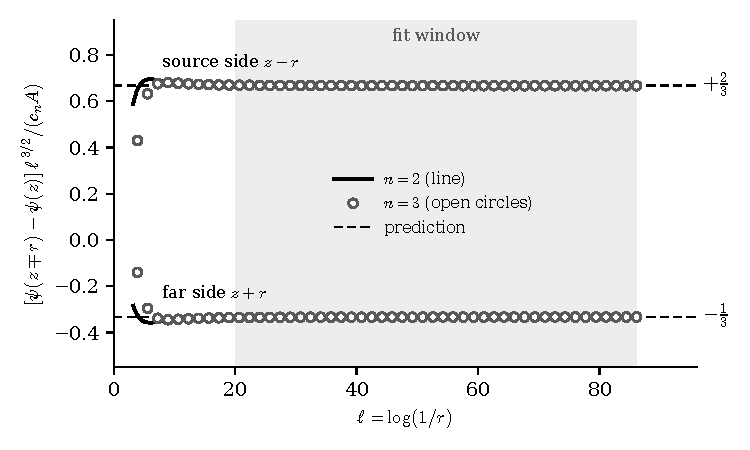
\includegraphics[width=0.8\textwidth]{numerics/fig_kink_split.pdf}
\caption{Generation-1 kink profile at $L=0.6$ (even ground state, $s=0$, $\lambda=-2.417$, $A=1.567$; P1, grading $\rho=1.15$ down to $r=10^{-40}$). Plotted: the one-sided excursions $[\psi(q\mp r)-\psi(q)]\ell^{3/2}/(c_nA)$ at $q=y_n=L-\log n$, with $\psi(q)$ from the cusp fit (the node value at $q$ itself is truncated). Dashed: the predicted split $+\frac23$ (source side) and $-\frac13$ (far side) of K3. Line: $n=2$; circles: $n=3$ (every 12th node). The two coincide because $D\approx-0.002$ and $\beta_2=\beta_3=0$ here, so the $O(1/\ell)$ correction nearly vanishes. Fitted limits: $0.66679$ and $-0.33335$ for both points. Data from the pre-registered run \texttt{k06\_r1.15.json}.}\label{fig:kink}
\end{figure}
